\documentclass[a4paper, 11pt]{report}
\usepackage{/Users/fgu/dev/projects/dotfiles/latex/paper}
\bibliography{/Users/fgu/dev/projects/dotfiles/latex/fabib}
\onehalfspacing

\title{\textbf{PhD notes and literature}}
\author{Fabian Gunzinger \\ Warwick Business School}
\date{\today}


\begin{document}

\maketitle
\tableofcontents
\newpage


\documentclass[a4paper, 11pt]{article}
\usepackage{/Users/fgu/dev/projects/dotfiles/latex/paper}
\bibliography{/Users/fgu/dev/projects/dotfiles/latex/fabib}
\onehalfspacing

\newcommand{\figdir}{../../output/figures}
\newcommand{\tabdir}{../../output/tables}

\title{\textbf{Entropy\footnote{This research was supported by Economic and Social Research Council grant number ES/V004867/1. WBS ethics code: E-414-01-20.}}}
\author{
    Fabian Gunzinger \\ Warwick Business School
    \and
    Neil Stewart \\ Warwick Business School
}
\date{\today}

\begin{document}

\maketitle

\tableofcontents

% !TEX root = ../entropy.tex

\section{Introduction}%
\label{sec:introduction}

Storyline:
\begin{itemize}

    \item This paper tests whether people save less in times when their lives
        are more chaotic. We define savings as ... and capture chaotic lives
        using ...

    \item Many people in UK and US struggle to save
        enough.

    \item This is well documented and thoroughly studied for retirement
        savings.

    \item But these are not only savings. People in UK and US also don't have
        enough to cover unexpected outlays.

    \item This could have important consequences: scarcity hypothesis - makes
        it harder to focus on important things (plan for retirement, focus on
        healthy lifestyle, support children, ...) and might lead to vicious
        cycle (less savings leading to increased risk of financial hardship
        leading to more stress leading to less savings...)

    \item This paper aims to start to fill gap and study short-term savings
        behaviour.

    \item In doing so, we aim to contribute to three literatures:

    \begin{itemize}
        \item Understanding ``rainy-day'' savings behaivour

        \item Understanding effect of behavioural entropy

        \item Use of high-frequency transaction data (itself a sub-literature of
            use of newly available large-scale datasets)
    \end{itemize}
\end{itemize}


% Literature:

% \citet{muggleton2020evidence} find that consumption entropy over categories
% correlates with financial distress.

% \citet{davenport2020spending} study the impact of COVID-19 on the spending and
% savings behaviour of MDB users.

% \citet{baker2021household} summarises literature that uses mass financial
% transaction data to study household financial behaviour.

% \citet{becker2017does} finds that access to a fintech money management app
% increases first-time savings and savings account balances among 65,000 customers
% of a large European bank but that update is negatively correlated with financial
% sophistication.

% \citet{colby2013savings} has useful literature review on short-term savings and
% suggests that subgoals can increase willingness to forego short-amounts in the
% present because they move the reference point in a prospect-theory framework.

% We use the following nomenclature throughout:
% \begin{description}
%     \item[user] individual
%     \item[tag] spending category
% \end{description}




% % !TEX root = ../entropy.tex

\section{Methods}%
\label{sec:methods}


\subsection{Dataset description}
\label{par:dataset_description}

We use data from Money Dashboard (MDB), a financial management app that allows
its users to link accounts from different banks to obtain an integrated view of
their
finances.\footnote{\href{https://www.moneydashboard.com}{https://www.moneydashboard.com}.}
The dataset contains more than 500 million transactions made between 2012 and
June 2020 by about 250,000 users, and provides information such as date,
amount, and description about the transaction as well as account and user-level
information.

The main advantages of the data for the study of consumer financial behaviour
are its high frequency, that it is automatically collected and updated and thus
less prone to errors and unaffected by biases that bedevil survey measures, and
that it offers a view of consumers' entire financial life across all their
accounts, rather than just a view of their accounts held at a single bank,
provided they added all their accounts to MDB. The main limitation is the
non-representativeness of the sample relative to the population as a whole.
Financial management apps are known to be used disproportionally by men,
younger people, and people of higher socioeconomic status
\citep{carlin2019generational}. Also, as pointed out in
\citet{gelman2014harnessing}, a willingness to share financial information with
a third party might not only select on demographic characteristics, but also
for an increased need for financial management or a higher degree of financial
sophistication. Because our analysis does not rely on representativeness, we do
not address this.\footnote{For an example of how re-weighing can be used to
mitigate the non-representative issue, see \citet{bourquin2020effects}.}


\subsection{Preprocessing and sample selection}%
\label{par:preprocessing_and_sample_selection}

We restrict our sample to users for whom we can observe a regular income, can
be reasonably sure that they have added all their bank account to MDB, and for
whom we observe at least six months of data. Table~\ref{tab:selection}
summarises the sample selection steps we applied to a 1 percent sample of the
raw data, associated data losses, and the size of our final sample. A detailed
description of the entire data cleaning and selection process is provided in
Appendix~\ref{sec:data}.

\begin{table}[H]
\caption{Sample selection}\label{tab:selection}
\begin{tabular}{lrrrr}
\toprule
                                                 &  Users & Accounts & Transactions & Value (\pounds M) \\
\midrule
                                      Raw sample & 24,163 &  123,625 &   59,647,019 &          11,209.7 \\
                       At least 6 months of data & 21,508 &  117,000 &   59,088,076 &          11,116.8 \\
                               No missing months & 18,550 &   98,513 &   51,252,412 &           9,606.4 \\
                      Account balances available & 14,714 &   85,590 &   44,163,629 &           8,618.7 \\
At least 5 debits totalling \pounds200 per month & 12,296 &   70,981 &   38,618,825 &           7,469.7 \\
                    At least one current account & 12,148 &   70,366 &   38,280,116 &           7,421.9 \\
            Income in 2/3 of all observed months &  9,963 &   60,151 &   33,270,455 &           6,490.2 \\
 Yearly income between \pounds5k and \pounds200k &  6,716 &   36,829 &   21,460,727 &           3,677.9 \\
            No more than 10 accounts in any year &  6,169 &   26,999 &   18,241,355 &           2,855.1 \\
      Debits of less than \pounds100k each month &  5,760 &   24,486 &   16,409,561 &           1,998.7 \\
                                    Final sample &  5,760 &   24,486 &   16,409,561 &           1,998.7 \\
\bottomrule
\end{tabular}

\end{table}



\subsection{Dependent variables}
\label{par:outcome_variable_}

Identifying savings transactions: We classify as payments into savings accounts
all savings account credits of \pounds5 or more that are not identified as
interest payments or automated "save the change" transfers (similarly for
debits).\footnote{While standing order transactions are unlikely to be related
to entropy in the short-run, we do not exclude such transactions since, best we
can tell, the only account for a small fraction of total transactions.} 

Dummy for savings txn in current month. Motivation: \citet{mps2018building} finds that
saving habit is often more important than amount saved.

Gross and net inflows into savings accounts in current month. We winsorise the
top end of the distribution at the 1 percent level.




\subsection{Spending profile}%
\label{par:variable_of_interest_}

\begin{itemize}
    \item Two ways to characterise spend profile: intra-period and
        inter-period. For proof-of-concept study, we focus on former, and on
        calendar month as period.\footnote{For intra-period characterisation,
        consistency over time will be particularly interesting. Might be able
    to capture this using Jensen-Shannon divergence.}
\end{itemize}


Measures of spending profiles:
\begin{itemize}
    \item Tag-based entropy

    \item Smoothed tag-based entropy

    \item Grocery-shops based entropy

    \item Composite measure based on PCA from combination of base entropy
        scores (similar to \citet{eagle2010network}
\end{itemize}


\paragraph{Tag-based entropy}%
\label{par:tag_based_entropy}

Our variable of interest is spending entropy, a measure of how predictable an
individual's spending pattern is at a given point in time, which we interpret
more broadly as a measure of the degree to which an individual's life is
chaotic. Entropy is a cornerstone of information theory, where it measures the
amount of information contained in an event. In the behavioural sciences,
behavioural entropy has recently been shown to predict the frequency of grocery
visits and the per-capita spend per visit \citep{guidotti2015behavioral}, the
amount of calories consumed \citep{skatova2019those}, and the propensity for
financial distress \citep{muggleton2020evidence}.

We calculate spending entropy using the formula proposed by
\citet{shannon1948mathematical}, which defines entropy as:\footnote{Shannon
    entropy is customarily denoted as $H$ following Shannon's own naming after
    Ludwig Boltzman's 1872 H-theorem in statistical mechanics, to which it is
analagous.}

\begin{equation}
\label{equ:entropy}
    H = -\sum{p_i}log(p_i),
\end{equation}

where $p_i$ is the probability that an individual makes a purchase in spending
category $i$, and $log$ is the base 2 logarithm.

\edit{We normalise $H$ by $log(N_{SC})$, the entropy of completely random shopping
    behaviour, so that it takes value between 0 and 1.\footnote{$log(N_{SC})$ is
    the probability of a completely random shopping pattern because for in this
case, for $N_{SC}$ different spending categories, we would have $p_i = 1 /
N_{SC}$ for each category $i$ so that $H = -N_{SC}p_ilog(p_i) = -log(p_i) =
log(N_{SC})$.}}

The higher the value of
entropy, the less predictable an individuals spending pattern.

To calculate entropy scores, we group spending into 9 spending categories (SC)
based on the classification used by Lloyds Banking Group as discussed in
\citet{muggleton2020evidence}. Also following that paper, we use additive
smoothing to calcualte probabilities to avoid taking logs of zeroes in cases
where an individual makes no purchases in a given spending category. We thus calculate $p_i$ as: 

\begin{equation}
    p_i = \frac{\text{Count of purchases in $SC_i$} + 1}{\text{Count of
    all purchases} + N_{SC}},
\end{equation}

where $N_{SC}$ is the total number of categories.

Issues from imperfect labelling of MDB data:
\begin{itemize}

    \item Transaction tagging in the MDB data is imperfect: about 20 percent of
        transactions have no tag.

    \item This creates two issues for entropy calculation.

    \item First, entropy scores of high-entropy individuals are biased
        downwards - relatively more than those of low-entropy individuals.
        Reason: missing tags are not random: more common transactions such as
        groceries or take-away purchases are more likely to be tagged ...

    \item All zero count-cases: ... Solution: require minimum number of txns in
        two different labels (for all categories we use to calculate entropy).
        Two to avoid 0 entropy cases that are unlikely to be genuine but
        probably artefacts of missing labelling.
        
\end{itemize}

\paragraph{Auto-tag-based entropy}
\label{par:auto_tag_entropy}

\begin{itemize}
    \item Use apriori algorithm

    \item minsup: minimum number of baskets a pattern is required to appear
        (else it's dropped)

    \item In our context: baseket is collection of auto tags with positive txsn
        counts in a user month, while pattern is pattern of such auto tags.

    \item Patterns also called 'representative baskets'.

    \item Algorithm steps (adapted from guidotti2015behavioural)

        \begin{itemize}
            \item Identify all patterns (representative baskets)

            \item Discard representative baskets that appear in fewer than
                minsup months we observe for a user. 

            \item Assign representative basked to each of the user's months.

            \item Calculate probabilities of observing a representative basked
                based on occurrences across all of a user's month. E.g. user
                with 5 months of data with representative baskets [1, 1, 2, 3,
                4] has representative basket probabilitis 2/5 for repr basket
                1, and 1/5 for repr baskets 2-4.

            \item Calculate user-leven entropy based on probabilities.
        \end{itemize}
\end{itemize}


\paragraph{Shopping-time based entropy}
\label{par:shopping_time_based_entropy}

We calculate entropy based on the probability of $(day of week, merchant)$
tuples, where we follow \citet{guidotti2015behavioral} and bin \textit{day of
week} into \textit{weekends} and \textit{weekday}, to reduce excessive
fluctuations. Because banks tend to process weekend transactions on Monday, as
shown in
Figure~\ref{fig:spending}, we cannot distinguish transactions made on Saturdays
or Sundays from those made on Mondays, and thus classify all of them as weekend
transactions.

We drop the about 25 percent of transactions for which we cannot identify a
merchant. The alternative would be leaving these transactions in the sample and
treating ``unknown merchant'' as a single merchant. But for user-months for
which the merchant is unknown for all transactions, this would lead to an
entropy score of 0, which is undesireable.

\paragraph{Grocery shop entropy}%
\label{par:grocery_shop_entropy}

We consider purchases at Tesco, Sainsbury's, Asda, Morrisons, Aldi, Co-op,
Lidl, Waitrose, Iceland, and Ocado, which have a combined market share of 96.5
percent.


\subsection{Control variables}%
\label{sub:control_variables}

We classify potential determinants of savings behaviour into \textit{financial behaviours},
\textit{financial planning}, and \textit{individual or household
characteristics}, a classification frequently used in policy research on
the financial wellbeing \citep{can2019improving,cfpb2017financial, mps2018building}.

Financial behaviour

\begin{itemize}
    \item Regular savings, dummy for 10 out of last 12 months

    \item Proportion of purchases paid with credit card. This is only about 6
        percent in our final sample, whereas it is 12 percent in the full
        sample.\footnote{Across the UK, the proportion of credit pard purchases
            is about 17 percent in a typical month \citep{ukfinance2021card}.
            The proportion in our data is likely lower because the sample is
        skewed towards more affluent individuals.}

    \item Month total and category spend (category spend for robustness)
\end{itemize}

Planning
\begin{itemize}
    \item Regular login, dummy for 1 / month in 10 out of last 12 months. Have
        login data for about 50 percent of sample, so best to work with full
        sample once I use it. Implement once I can do that. -- not yet
        implemented --
\end{itemize}

Individual and household characteristics
\begin{itemize}
    \item Gender

    \item Age

    \item Urban

    \item Region

    \item Year income, winsorised at the 1 percent level. We include
        year-rather than month-income because the latter can be quite variable
        (e.g. irregular work, changing jobs, etc.), and we assume people to
        base their consumption on their annual income. (Could test this in
        appendix: is correlation between annual and spend stronger than between
        monthly and spend?)

    % \item Month income, winsorised at top 1 percent-level.

    \item Regular income, dummy for 10 out of last 12 months

    \item Month income std -- not implemented yet --

    \item Income current month, dummy for month income > 0

    \item Has children, imperfect -- not yet implemented --

    \item Index of multiple deprivations from nspl -- not implemented yet --

    \item Received benefits

    \item Receives pension

    \item Housing tenure: mortgage, rent, other (owning outright implied)

    \item Takes out (payday) loan

    \item Total balance or balance / avg. month spend -- not yet implemented --
\end{itemize}




\subsection{Summary statistics}%
\label{par:summary_statistics}

Table~\ref{tab:sumstats} provides summary statistics.


% Table created by stargazer v.5.2.3 by Marek Hlavac, Social Policy Institute. E-mail: marek.hlavac at gmail.com
% Date and time: Mon, Sep 26, 2022 - 09:41:15
\begin{tabular}{@{\extracolsep{5pt}}lccccccc} 
\\[-1.8ex]\hline 
\hline \\[-1.8ex] 
Statistic & \multicolumn{1}{c}{Mean} & \multicolumn{1}{c}{St. Dev.} & \multicolumn{1}{c}{Min} & \multicolumn{1}{c}{Pctl(25)} & \multicolumn{1}{c}{Median} & \multicolumn{1}{c}{Pctl(75)} & \multicolumn{1}{c}{Max} \\ 
\hline \\[-1.8ex] 
Month income & 2.77 & 2.23 & 0.00 & 1.45 & 2.18 & 3.43 & 13.69 \\ 
Has income in month & 0.98 & 0.13 & 0 & 1 & 1 & 1 & 1 \\ 
Has savings & 0.50 & 0.50 & 0 & 0 & 1 & 1 & 1 \\ 
Month spend & 2.90 & 2.50 & 0.20 & 1.37 & 2.20 & 3.49 & 16.05 \\ 
Age & 35.72 & 9.74 & 18 & 28 & 34 & 42 & 65 \\ 
Female & 0.43 & 0.49 & 0 & 0 & 0 & 1 & 1 \\ 
Urban & 0.85 & 0.36 & 0 & 1 & 1 & 1 & 1 \\ 
Unique categories (9) & 7.84 & 1.05 & 1 & 7 & 8 & 9 & 9 \\ 
Unique categories (48) & 16.54 & 4.13 & 1 & 14 & 16 & 19 & 35 \\ 
Unique categories (Merchants) & 26.78 & 9.35 & 2 & 20 & 26 & 33 & 85 \\ 
\hline \\[-1.8ex] 
\end{tabular} 


Figure~\ref{fig:entropy_kdes}
\begin{figure}[H]
    \center \newcommand\width{\textwidth} \caption{Entropy distributions}
    \label{fig:entropy_kdes}
    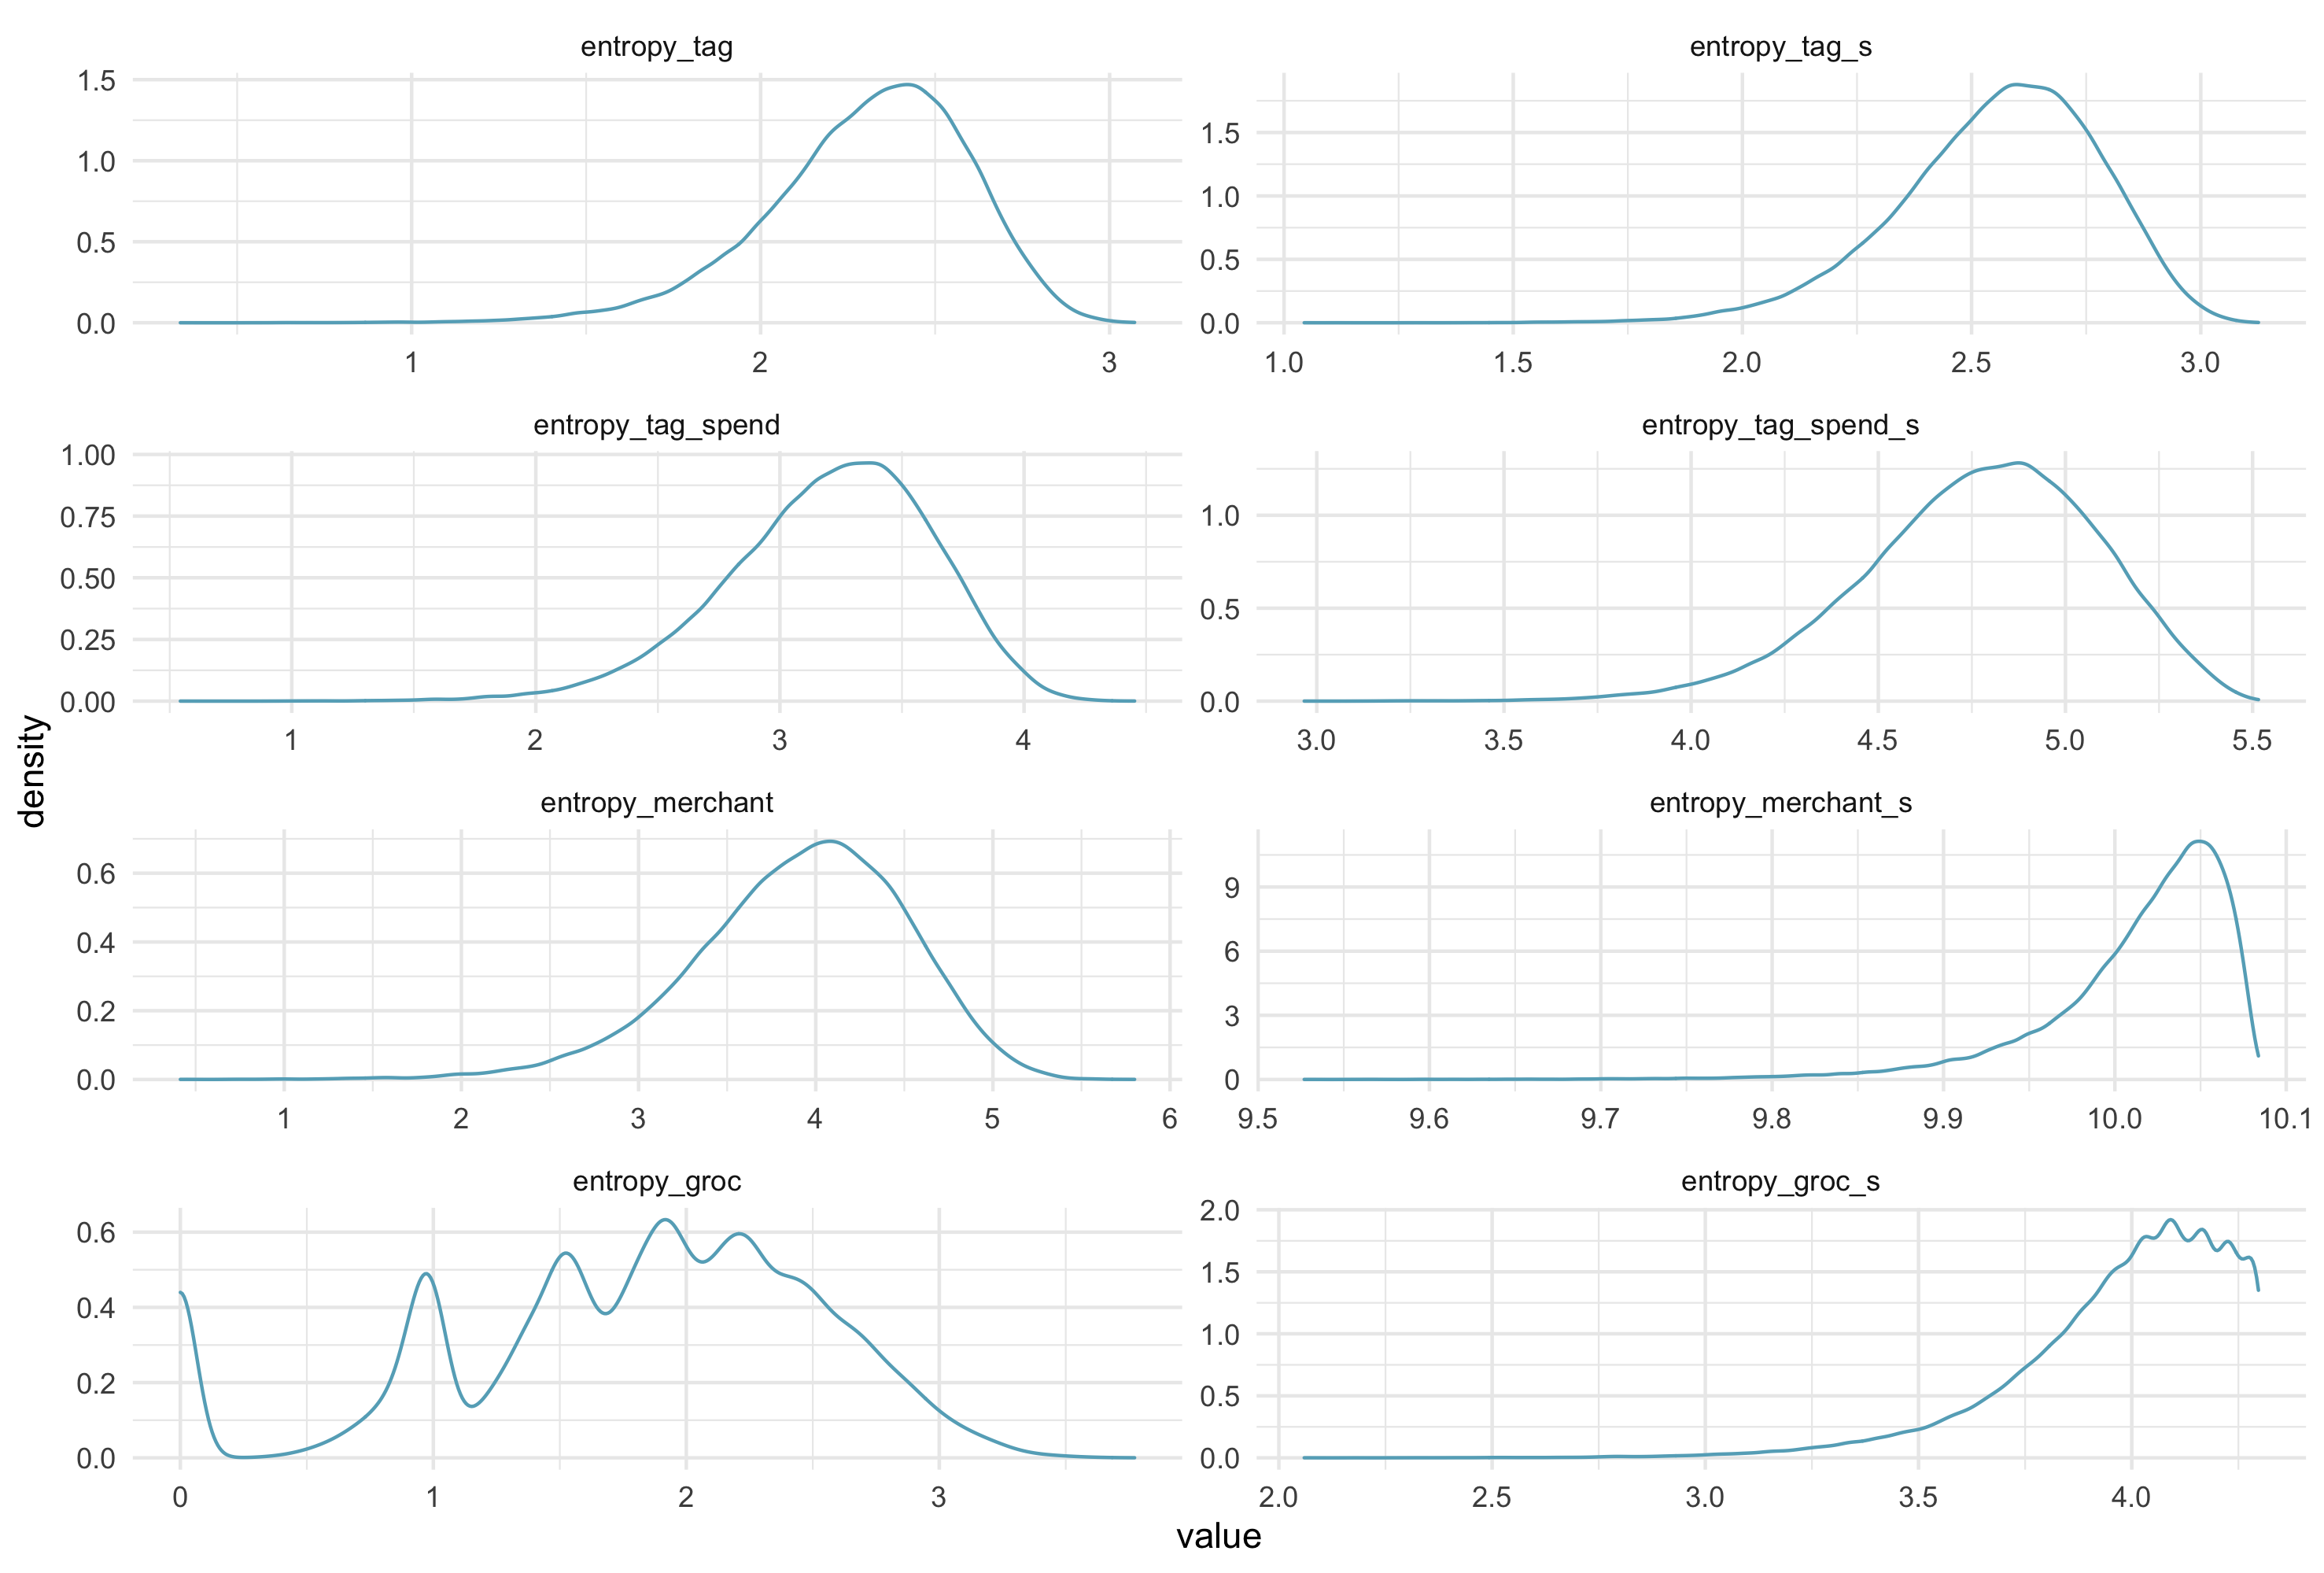
\includegraphics[width=\width]{\figdir/entropy_kdes.png}
    \fignote{\width}{}
\end{figure}




\subsection{Model specification}%
\label{par:model_specification}

We estimate models of the form: 

\begin{equation}
    s_{i,t} = \alpha_i + \lambda_t + \beta H_{i,t} + x^\prime_{i,t} \delta +
    \epsilon_{i,t},
\end{equation}

where $s_{i,t}$ is an indicator variable equal to one if individual $i$ made
one or more transfers to any of their savings account in month $t$ and zero
otherwise, $H_{it}$ is $i$'s spending entropy in month $t$, $x_{i,t}$ a vector
of control variables, $\alpha_i$ an individual fixed effect, $\lambda_t$ a
calendar month fixed effect, and $\epsilon_{i, t}$ the error term.

Issues to think about:
\begin{itemize}
    \item Unbalanced panel is not random - people using MDB for longer are
        different. Should we just use first x months for every user? E.g. first
        year?
\end{itemize}



% % !TEX root = ../entropy.tex

\section{Spending profiles predict emergency savings}%
\label{sec:results}

Table~\ref{tab:main} shows the effect of entropy on the probability of building
emergency savings in a given month. Columns (1)-(3) show results for unsmoothed
entropy based on 9 categories, 48 categories, and merchant names, respectively.
Columns (4)-(6) show results for smoothed entropy based on the same variables.
All models include user and year-month fixed effects, and standard errors are
clustered at the user-level. 95\% confidence intervals are shown in
brackets.\footnote{In line with an emerging consensus for how to avoid
    over-reliance on statistical significance, we deliberately do not show
    significance stars in our regression tables and instead emphasise the
    implications of the bounds of the confidence intervals when discussing our
    results. For two recent discussions, see \citet{imbens2021statistical,
romer2020praise}.}

Results for unsmoothed entropy suggest that a one standard-deviation increase
in spending entropy is associated with an increase in the probability of a user
making at least one transfer into their savings accounts of between 1.1 and 2.3
percentage points -- an effect equal to an increase in monthly income of
between \pounds1000 and \pounds2000. Combined, the results in the three columns
present very strong evidence that entropy captures something about users's
spending distribution that is related to their likelihood for making payments
into their savings accounts. Furthermore, entropy variables defined based on a
larger number of unique categories, that allow for a more precise segmentation
of spending behaviour, capture features of spending behaviour that are as
strongly or more strongly related to savings behaviour as monthly income.

The results for smoothed entropy are similar but a tend to be smaller in
magnitude, and -- together -- also provide strong evidence that smoothed
entropy captures features of spending behaviour that is related to savings
behaviour in a statistically significant and economically relevant way. The
main difference to the results for unsmoothed entropy is the reversal of the
sign of the coefficients: across all three measures, an increase in entropy is
estimated to be associated with a decrease in the likelihood of any savings
transactions. The effect of the measure based on 9 categories is not
meaningfully different from zero, but the estimates for the measures based on
48 categories and merchants are almost identical and suggest that the magnitude
of the effect is between 1.2 and 2.1 percentage points -- equalling the effect
of a reduction of monthly income of between \pounds1000 and \pounds2000.

\begin{landscape}
    \begin{table}[ht]
        \centering\scriptsize
        \caption{Effect of entropy on P(savings transactions)}
        \label{tab:main}
        
\begin{table}[htbp]
   \centering
   \tiny
   \begin{threeparttable}[b]
      \caption{\label{tab:reg_has_inflows_main} Effect of entropy on P(transfer into savings accounts)}
      \begin{tabular}{lcccccc}
         \tabularnewline \midrule \midrule
         Model:                     & (1)             & (2)             & (3)             & (4)              & (5)              & (6)\\  
         \midrule
         \emph{Variables}\\
         Entropy (9 cats)           & 0.016$^{***}$   &                 &                 &                  &                  &   \\   
                                    & [0.013; 0.019]  &                 &                 &                  &                  &   \\   
         Entropy (48 cats)          &                 & 0.029$^{***}$   &                 &                  &                  &   \\   
                                    &                 & [0.025; 0.033]  &                 &                  &                  &   \\   
         Entropy (merchant)         &                 &                 & 0.032$^{***}$   &                  &                  &   \\   
                                    &                 &                 & [0.029; 0.036]  &                  &                  &   \\   
         Entropy (9 cats, smooth)   &                 &                 &                 & -0.008$^{***}$   &                  &   \\   
                                    &                 &                 &                 & [-0.010; -0.006] &                  &   \\   
         Entropy (48 cats, smooth)  &                 &                 &                 &                  & -0.023$^{***}$   &   \\   
                                    &                 &                 &                 &                  & [-0.025; -0.020] &   \\   
         Entropy (merchant, smooth) &                 &                 &                 &                  &                  & -0.019$^{***}$\\   
                                    &                 &                 &                 &                  &                  & [-0.021; -0.016]\\   
         Month spend                & 0.009$^{***}$   & 0.009$^{***}$   & 0.008$^{***}$   & 0.009$^{***}$    & 0.008$^{***}$    & 0.007$^{***}$\\   
                                    & [0.009; 0.010]  & [0.008; 0.009]  & [0.008; 0.009]  & [0.009; 0.010]   & [0.007; 0.009]   & [0.007; 0.008]\\   
         Month income               & 0.012$^{***}$   & 0.012$^{***}$   & 0.012$^{***}$   & 0.012$^{***}$    & 0.011$^{***}$    & 0.011$^{***}$\\   
                                    & [0.011; 0.013]  & [0.011; 0.013]  & [0.011; 0.013]  & [0.011; 0.013]   & [0.011; 0.012]   & [0.010; 0.012]\\   
         Has income in month        & 0.086$^{***}$   & 0.084$^{***}$   & 0.083$^{***}$   & 0.087$^{***}$    & 0.085$^{***}$    & 0.086$^{***}$\\   
                                    & [0.077; 0.094]  & [0.075; 0.092]  & [0.074; 0.091]  & [0.079; 0.096]   & [0.076; 0.093]   & [0.078; 0.095]\\   
         Income variability         & 0.001$^{*}$     & 0.001$^{*}$     & 0.001$^{*}$     & 0.001$^{*}$      & 0.001$^{*}$      & 0.000\\   
                                    & [-0.000; 0.001] & [-0.000; 0.001] & [-0.000; 0.001] & [-0.000; 0.001]  & [-0.000; 0.001]  & [-0.000; 0.001]\\   
         \midrule
         \emph{Fixed-effects}\\
         User                       & Yes             & Yes             & Yes             & Yes              & Yes              & Yes\\  
         Year-month                 & Yes             & Yes             & Yes             & Yes              & Yes              & Yes\\  
         \midrule
         \emph{Fit statistics}\\
         Observations               & 1,043,727       & 1,043,727       & 1,043,416       & 1,043,727        & 1,043,727        & 1,043,416\\  
         R$^2$                      & 0.45368         & 0.45395         & 0.45410         & 0.45363          & 0.45415          & 0.45410\\  
         Within R$^2$               & 0.00719         & 0.00768         & 0.00807         & 0.00709          & 0.00805          & 0.00808\\  
         \midrule \midrule
         \multicolumn{7}{l}{\emph{Clustered (User) co-variance matrix, 95\% confidence intervals in brackets}}\\
         \multicolumn{7}{l}{\emph{Signif. Codes: ***: 0.01, **: 0.05, *: 0.1}}\\
      \end{tabular}
   \end{threeparttable}
\end{table}



        \tabnote{1.2\textwidth}{Results from estimating
            Equation~\ref{equ:model}. The
                dependent variable in all columns is a dummy variable
                indicating whether a
                    user made at least one transaction into any of their
                    savings accounts in a
                given period. \regtabinfo}
    \end{table}
\end{landscape}

As discussed in Section~\ref{sub:estimation}, these results are not due to
reverse causality. While we might think that making a savings transactions
might change some or all of the components of entropy discussed in
Section~\ref{sub:spending_profiles} -- the number of unique spending categories
with positive frequency count, the standard deviation of these counts, and the
total number of spend transactions -- and thus change entropy, this is not the
case because of the way we define entropy and savings, and the way spending
transactions are categorised. We define entropy based on all current account
debits that are identified as spends, while we define savings transactions as
the sum of all savings accounts credits. If a user transfers money from their
current account to their savings account, this will be identified as a savings
transaction, but be identified as a transfer on their current account and thus
not considered when calculating their entropy score.

The estimates of our control variables are largely as expected, with the
exception of monthly spend, which one might have expected to be negatively
correlated with savings. Also, it is evident that the strongest predictor among
the included controls for whether a user makes any savings transfer is whether
they receive any income in that month. Income variability, in contrast, is not
correlated with savings behaviour in any economically significant way,
suggesting that people with variable incomes do not build savings cushions for
periods where they have no income.

Overall, the effect of entropy in spending profiles is statistically and
economically significant, and robust across different definitions. In other
words, the scores seem to pick up a feature of the spending distribution that
is predictive of savings behaviour. The obvious question raised by the results
is why smoothing entropy scores flips the direction of the effect of entropy.
We address this next.


\subsection{Why does smoothing flip the direction of the effect}%
\label{sub:why_does_smoothing_flip_the_direction_of_the_effect}

One way to think about the sign change in Table~\ref{tab:main} is to realise
that it implies that at least for some individuals, the relative rank of
smoothed and unsmoothed entropy must differ considerably -- there must be some
individuals that have low unsmoothed entropy but high smoothed entropy or some
that have high unsmoothed entropy and low smoothed entropy or both.
Understanding who those individuals are might thus help us understand the sign
flip.

To understand rank differences between unsmoothed and smoothed entropy scores
it is useful to rewrite Equation~\ref{equ:entropy} in a way that makes it easy
to see its component parts. Remember from Section~\ref{sub:spending_profiles}
that $f_c$ is the number of transactions made by a user in a given period in
spending category $c$, $\setc$ the set of all spending categories, and $F$ the
total number of transactions made by a given user in a given period.
Additionally, let $\setcp = \{c: f_c > 0\}$ be the set of all spending
categories with positive frequency counts (i.e.  with at least one transaction)
and $\setcz = \{c: f_c = 0\}$ the set of all spending categories with a zero
frequency count, so that $\setc = \setcz \cup \setcp$. Then, using our
definitions of unsmoothed and smoothed probabilities, we can write unsmoothed
entropy as

\begin{equation}
\label{equ:entropy_us}
H = -\sum_{c \in \setcp}{\left(\frac{f_c}{F}\right)
log\left(\frac{f_c}{F}\right)},
\end{equation}

and smoothed entropy as:

\begin{equation}
\label{equ:entropy_s}
H^s = -\sum_{c \in \setcp}{\left(\frac{f_c + 1}{F + |\setc|}\right)
log\left(\frac{f_c + 1}{F + |\setc|}\right)}
- |\setcz|\left(\frac{1}{F + |\setc|}\right)
log\left(\frac{1}{F + |\setc|}\right),
\end{equation}

\noindent where the size of set $\setcz$, $|\setcz|$, is the number of all
spending categories in which a user makes no transactions in the period.
These expressions make clear that, by definition, unsmoothed entropy is a
function of frequency counts of categories with positive counts only while
smoothed entropy has two parts: the sum over all additively smoothed frequency
counts of categories with positive counts, plus the same sum for additively
smoothed probabilities of categories with zero counts, which reduces to a
constant term that is multiplied by the number of such categories.

The expressions also make transparent the three main components of both types
of entropy that are determined by user behaviour. The first is the number of
spending categories with a non-zero frequency count, $|\setcp|$, which
determines the number of elements summed over in Equation~\ref{equ:entropy_us},
and partitions the categories into either contributing to the sum on the left
hand side of Equation~\ref{equ:entropy_s} or -- given that for an exogenously
fixed $|\setc|$, $|\setcz| = |\setc \backslash \setcp|$ -- to the constant term
on the right hand side. The second component is the variation of the frequency
counts, $f_c$, and the third component is the number of total spend
transactions, $F = \sum_{\setc}f_c$. Together, these two elements determine the probabilities
associated with a spend transaction occurring in a given category. The number
of total spending categories, $|\setc|$, also determines smoothed entropy and,
implicitly, also unsmoothed entropy since it ``scales'' the number of
categories with a positive frequency count, $|\setcp|$, as a given number of
spending transactions are categorised into finer or coarser categories. But it
is exogenously given and does not depend on user behaviour.

\begin{figure}[ht]
    \centering 
    \caption{Effect of smoothing on entropy}
    \label{fig:scatter_facets}
    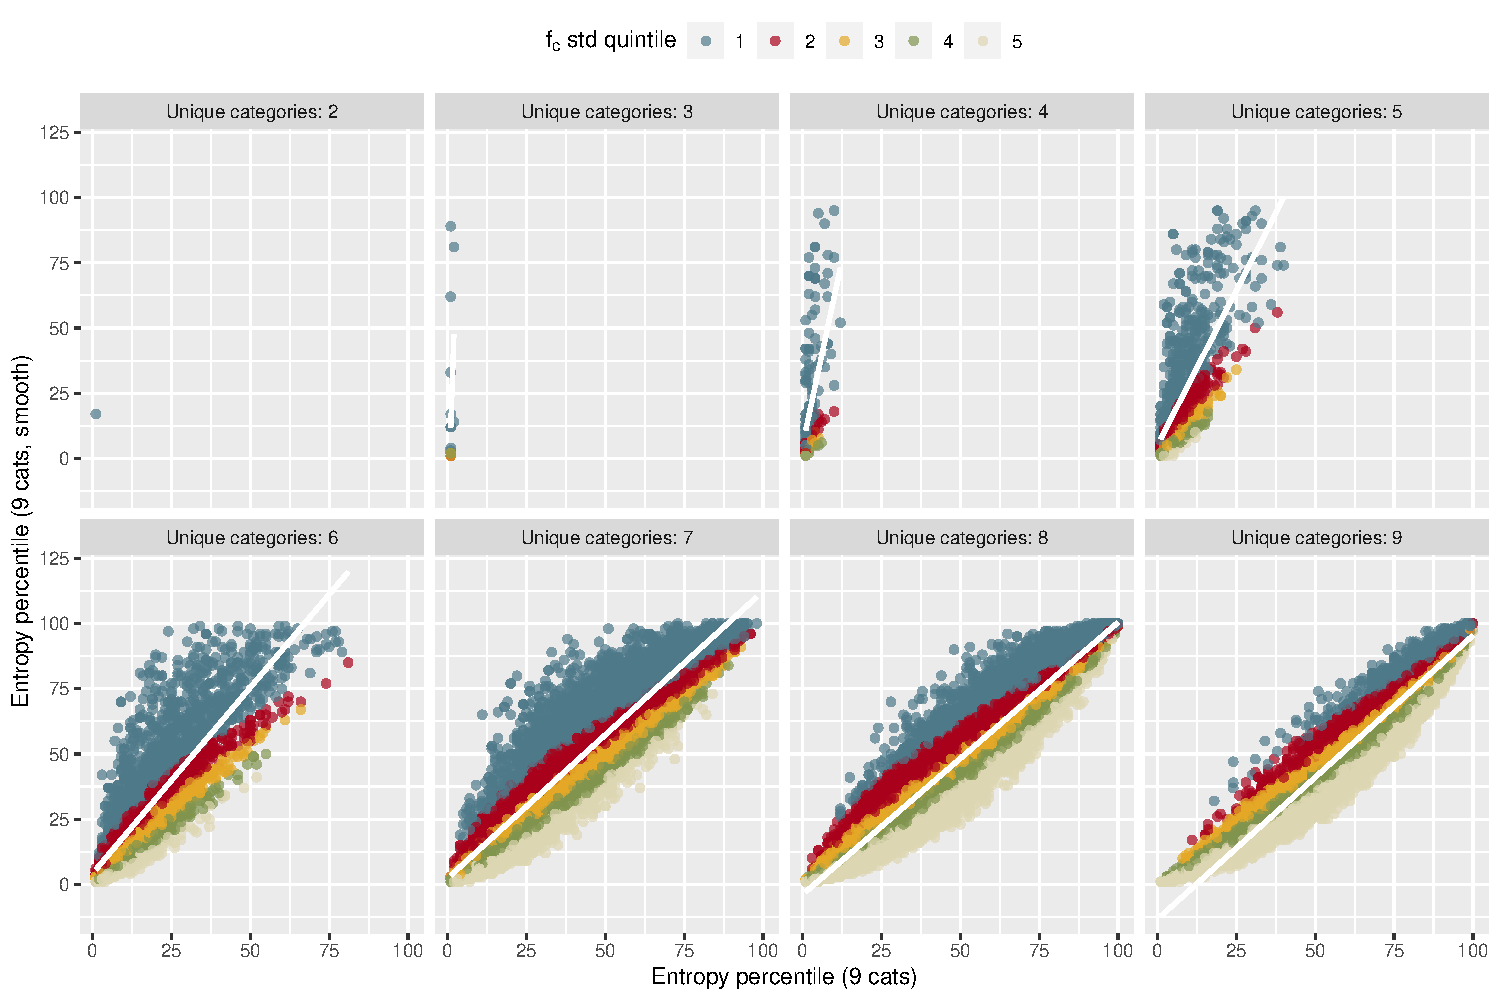
\includegraphics[width=\textwidth]{\figdir/scatter_facet_std_tag_q.pdf}
    \fignote{\textwidth}{Percentile ranks of 9-category-based unsmoothed and
    smoothed entropy separated by the number of categories with positive
frequency counts. White reference lines indicate equal percentile ranks;
colours, frequency count standard deviation quintiles. Figure is based on a
10\% sample of the dataset used for analysis. There are only 8 panels since
there are cases where a user has spends in only a single category.}
\end{figure}

These components help us reason about rank differences between unsmoothed and
smoothed entropy. From equations~\ref{equ:entropy_us} and~\ref{equ:entropy_s}
we can see that the first part of smoothed entropy that sums over all spending
categories with positive frequency counts is very similar to the entire
expression of unsmoothed entropy -- it is that same expression but with
additively smoothed probabilities. Hence, all else equal, the higher the number
of categories with positive counts, the more smoothed entropy is determined by
that first part, and the more similar it will be to unsmoothed entropy. As a
result, we would expect to find large (rank) differences between entropy scores
among cases with few positive-counts categories. Furthermore, given that
unsmoothed entropy is increasing in the number of categories with positive
counts, we expect these cases to have relatively low unsmoothed entropy.

Given that we expect high rank difference cases to make spends across a small
number of categories, and expect these cases to have low unsmoothed entropy,
high rank differences will occur among the subset of those cases that have high
smoothed entropy. Remember from Section~\ref{sub:spending_profiles} that
entropy is higher the more equal the spending category probabilities are.
Hence, for a given number of zero-count categories, smoothed entropy will be
higher if the (additively smoothed) probabilities of all positive-count
categories are close to the (additively smoothed) probabilities of the
zero-count categories, which will be the case (i) if there are few overall
transactions, such that frequency counts ($f_c$) are close to zero and (ii) if
the counts are similar.

Figure~\ref{fig:scatter_facets} visualises this entire line of reasoning for
our 9-category based entropy variable: it shows scatter plots of the percentile
ranks of unsmoothed and smoothed entropy with a reference line indicating
identical rank, separated by the number of categories with positive frequency
counts and coloured based on the quintile of the frequency count standard
deviation.\footnote{Colouring based on the quintile of the total number of
transactions leads to a very similar plot and is thus not shown.} First,
ignoring the colouring and focusing on the shape of the dots only we can see
that, as expected, the relationship between the two entropy measures is tighter
the higher the number of non-zero spending categories is. Cases with large
entropy rank differences are thus to be found among cases with fewer positive
spend categories. Among these, the colouring makes clear that, as expected, the
cases with the largest rank differences -- those with the furthest vertical
difference to the reference line -- have low variation in their frequency
counts. However, it is also clear that the reverse is not true: there are cases
with low count frequency variation that experience little or even a negative
rank difference. Furthermore, among cases with a higher number of categories
with positive counts, cases with a very high variation in frequency counts can
also experience quite large rank differences, albeit in the opposite direction.
Hence, while counts variation is some help in identifying cases with high
entropy rank differences, it does not do so perfectly.

One reason the relationship is not perfect is that while cases with few total
transactions that are evenly spread across a small number of categories will
have high smoothed entropy, such will also have high unsmoothed entropy. What
we are looking for, more precisely, are cases where this pattern holds broadly,
but that also have a small number of frequency counts that dominate the others
but are still relatively close to zero. This would lead to low unsmoothed
entropy (because of the dominant counts) but high smoothed entropy (because all
counts are still relatively close to zero, so that the additively smoothed
distribution resembles a uniform distribution). Further research will be
necessary to more fully classify such cases, and to inquire what it is about
their behaviour that might be related to savings behaviour.


\subsection{Is entropy informative beyond its component parts?}%
\label{sub:is_entropy_informative_beyond_its_component_parts_}

Another question that arises once we think of entropy as comprising three main
component parts is whether its non-linear nature captures anything about the
relationship between spending and saving behaviour that is not captured already
by the three simpler components. 

\begin{landscape}
\begin{table}[ht]
\centering\scriptsize
\caption{Controlling for components}
\label{tab:components}

\begin{table}[htbp]
   \centering
   \tiny
   \begin{threeparttable}[b]
      \caption{\label{tab:reg_has_inflows_comp} Controlling for entropy components}
      \begin{tabular}{lcccc}
         \tabularnewline \midrule \midrule
         Model:                    & (1)             & (2)             & (3)              & (4)\\  
         \midrule
         \emph{Variables}\\
         Entropy (48 cats)         & 0.029$^{***}$   & 0.013$^{***}$   &                  &   \\   
                                   & [0.025; 0.033]  & [0.006; 0.021]  &                  &   \\   
         Entropy (48 cats, smooth) &                 &                 & -0.023$^{***}$   & -0.028$^{***}$\\   
                                   &                 &                 & [-0.025; -0.020] & [-0.034; -0.022]\\   
         Unique categories         &                 & 0.004$^{***}$   &                  & 0.004$^{***}$\\   
                                   &                 & [0.003; 0.005]  &                  & [0.004; 0.005]\\   
         Category counts std.      &                 & 0.002           &                  & -0.015$^{***}$\\   
                                   &                 & [-0.001; 0.006] &                  & [-0.018; -0.011]\\   
         Number of spend txns      &                 & 0.000$^{***}$   &                  & 0.001$^{***}$\\   
                                   &                 & [0.000; 0.001]  &                  & [0.001; 0.001]\\   
         Month spend               & 0.009$^{***}$   & 0.005$^{***}$   & 0.008$^{***}$    & 0.005$^{***}$\\   
                                   & [0.008; 0.009]  & [0.004; 0.006]  & [0.007; 0.009]   & [0.005; 0.006]\\   
         Month income              & 0.012$^{***}$   & 0.011$^{***}$   & 0.011$^{***}$    & 0.011$^{***}$\\   
                                   & [0.011; 0.013]  & [0.010; 0.012]  & [0.011; 0.012]   & [0.010; 0.012]\\   
         Has income in month       & 0.084$^{***}$   & 0.079$^{***}$   & 0.085$^{***}$    & 0.078$^{***}$\\   
                                   & [0.075; 0.092]  & [0.070; 0.087]  & [0.076; 0.093]   & [0.070; 0.087]\\   
         Income variability        & 0.001$^{*}$     & 0.000           & 0.001$^{*}$      & 0.000\\   
                                   & [-0.000; 0.001] & [-0.000; 0.001] & [-0.000; 0.001]  & [-0.000; 0.001]\\   
         \midrule
         \emph{Fixed-effects}\\
         User                      & Yes             & Yes             & Yes              & Yes\\  
         Year-month                & Yes             & Yes             & Yes              & Yes\\  
         \midrule
         \emph{Fit statistics}\\
         Observations              & 1,043,727       & 1,043,727       & 1,043,727        & 1,043,727\\  
         R$^2$                     & 0.45395         & 0.45498         & 0.45415          & 0.45515\\  
         Within R$^2$              & 0.00768         & 0.00956         & 0.00805          & 0.00986\\  
         \midrule \midrule
         \multicolumn{5}{l}{\emph{Clustered (User) co-variance matrix, 95\% confidence intervals in brackets}}\\
         \multicolumn{5}{l}{\emph{Signif. Codes: ***: 0.01, **: 0.05, *: 0.1}}\\
      \end{tabular}
   \end{threeparttable}
\end{table}



\tabnote{1.5\textwidth}{\regtabinfo}
\end{table}
\end{landscape}

We can test this by checking whether the relationship between spending entropy
and the probability of making a savings transaction remains economically and
statistically significant once we control for the three components. Columns (1)
and (3) in Table~\ref{tab:components} replicate the results for the 48-category-based
unsmoothed and smoothed entropy measures presented in Table~\ref{tab:main} for
reference. In columns (2) and (4) we additionally control for the three entropy
components. Including these components has some effect: the coefficients change
slightly -- decreasing in absolute magnitude in the case of unsmoothed entropy,
increasing in the case of smoothed entropy -- while the width of the confidence
intervals about double in both cases, reflecting the strong collinearity amount
the component and entropy. However, both coefficients remain statistically
significant and their confidence intervals cover values that are also
economically significant. Hence, the results make clear that the results in
Table~\ref{tab:main} cannot be attributed simply to the effect of one or more
of entropy's simple components.






\printbibliography

\end{document}



- Does entropy predict savings behaviour? 

- Entropy: over categories and time

- Savings behaviour: regularity of savings, amount of savings]b




%%%%%%%%%%%%%%%%%%%%%%%%%%%%%%%%%%%%%%%%%%%%%%%%%%%%%%%%%%%%%%%%%%%%%%%%%%%%%%%
%%%%%%%%%%%%%%%%%%%%%%%%%%%%%%%%%%%%%%%%%%%%%%%%%%%%%%%%%%%%%%%%%%%%%%%%%%%%%%%
%%%%%%%%%%%%%%%%%%%%%%%%%%%%%%%%%%%%%%%%%%%%%%%%%%%%%%%%%%%%%%%%%%%%%%%%%%%%%%%
						\part{Financial behaviour}
%%%%%%%%%%%%%%%%%%%%%%%%%%%%%%%%%%%%%%%%%%%%%%%%%%%%%%%%%%%%%%%%%%%%%%%%%%%%%%%
%%%%%%%%%%%%%%%%%%%%%%%%%%%%%%%%%%%%%%%%%%%%%%%%%%%%%%%%%%%%%%%%%%%%%%%%%%%%%%%
%%%%%%%%%%%%%%%%%%%%%%%%%%%%%%%%%%%%%%%%%%%%%%%%%%%%%%%%%%%%%%%%%%%%%%%%%%%%%%%


%%%%%%%%%%%%%%%%%%%%%%%%%%%%%%%%%%%%%%%%%%%%%%%%%%%%%%%%%%%%%%%%%%%%%%%%%%%%%%%
%%%%%%%%%%%%%%%%%%%%%%%%%%%%%%%%%%%%%%%%%%%%%%%%%%%%%%%%%%%%%%%%%%%%%%%%%%%%%%%
						\chapter{Why it matters}
%%%%%%%%%%%%%%%%%%%%%%%%%%%%%%%%%%%%%%%%%%%%%%%%%%%%%%%%%%%%%%%%%%%%%%%%%%%%%%%
%%%%%%%%%%%%%%%%%%%%%%%%%%%%%%%%%%%%%%%%%%%%%%%%%%%%%%%%%%%%%%%%%%%%%%%%%%%%%%%

See \citet{agarwal2017shapes,greenberg2019financial} for literature reviews.


\paragraph{Why does it matter?}
\begin{itemize}
	\item Important implications for (financial-) wellbeing \citep{lynch2011introduction}

	\item Undersaving for retirement \citep{benartzi2013behavioral}.
	\begin{itemize}
		\item \citet{scott2020can} argue that given mortality risk and low interest rates both at an absolute level and relative to discount rate, not saving a lot (or at all) can be rational for lower income people.
	\end{itemize}

	\item Inability to cover unexpected expenses \citep{lusardi2011financially}

	\item Inability to cover regular living expenses

	\item Might lead to scarcity and even more far-reaching consequences.
\end{itemize}



%%%%%%%%%%%%%%%%%%%%%%%%%%%%%%%%%%%%%%%%%%%%%%%%%%%%%%%%%%%%%%%%%%%%%%%%%%%%%%%
%%%%%%%%%%%%%%%%%%%%%%%%%%%%%%%%%%%%%%%%%%%%%%%%%%%%%%%%%%%%%%%%%%%%%%%%%%%%%%%
					\chapter{Behaviours}
%%%%%%%%%%%%%%%%%%%%%%%%%%%%%%%%%%%%%%%%%%%%%%%%%%%%%%%%%%%%%%%%%%%%%%%%%%%%%%%
%%%%%%%%%%%%%%%%%%%%%%%%%%%%%%%%%%%%%%%%%%%%%%%%%%%%%%%%%%%%%%%%%%%%%%%%%%%%%%%

%%%%%%%%%%%%%%%%%%%%%%%%%%%%%%%%%%%%%%%%%%%%%%%%%%%%%%%%%%%%%%%%%%%%%%%%%%%%%%%
\section{Saving}
%%%%%%%%%%%%%%%%%%%%%%%%%%%%%%%%%%%%%%%%%%%%%%%%%%%%%%%%%%%%%%%%%%%%%%%%%%%%%%%

\begin{itemize}

	\item See introduction of \citet{browning1996household} for Keynes' eight motives for why people save.

	\item Economics literature on saving:
	\begin{itemize}
		\item \citet{browning2001life}: summary of life-cycle model.

		\item \citet{browning1996household}: summary of savings literature (find newer version).

		\item \citet{lusardi2000explaining}: explaining why households save so little.

		\item \citet{thaler1990anomalies}: on savings anomalies.

		\item \citet{thaler1994psychology}: psychology and savings policies.

		\item Suggestions for how savings can be incentivised \citep{thaler1994psychology} and effects of effects of incentivised savings (like IRAs) \citep{middleton2018lifting} and references therein.

		\item \citet{blumenstock2018defaults} Table A1 (in blumenstock2018defaultsWP) for overview of default savings effects.

		\item \citet{blumenstock2018defaults}
		\begin{itemize}
			\item Test the effect of defaults on precautionary savings and mechanism analysis.

			\item Randomly assign about 1000 employees to either 0\% or 5\% of their salary being automatically transferred to a savings account by default, and to a 0, 25, and 50 percent employer matching incentive (i.e. 2 x 3 design).

			\item Effects of defaults, key findings: 1) employees in the default condition were 40 percentage points more likely to contribute to the account. 2) The default assignment increases savings by about as much as a 50 percent employer match. 3) Long term effects: 45\% or all participants elected to keep contributing to the account once financial incentives were removed, with participation 25\% higher in the default group. (Overall, this suggests habit formation in savings behaviour). Also, default group felt more financially secure, and 2 years later their savings balance remained higher.

			\item Why do defaults work? Possible channels are 1) endorsement effect, 2) real or perceived switching costs, 3) mental cost of forming a financial plan (due to complexity), 4) unawareness of election, or lack of salience of switching option, 5) present biasedness (switching involves immediate cost and future benefits). They find that their results are mainly driven by mental cost of forming a plan and present biasedness.

			\item Appendix B has a nice simple framework of their setting based on \citet{o1999doing}.
		\end{itemize}
	\end{itemize}


	\item Retirement savings:
	\begin{itemize}
		\item laibson2020aea1 - laibson2020aea4 (and entire \href{https://www.aeaweb.org/webcasts/2020/aea-afa-joint-luncheon-nudges-are-not-enough}{talk}) for great overview of literature on retirement savings and on positive effect of defaults on proxy outcomes and neutral/very small effects on welfare (semblance of success. Basic point: the effects of defaults on retirement savings are very small. Reason: people in the control group seem to catch up over time, and there is a huge amount of leakage out of retirement savings accounts. Suggestions from new models: make savings in the US mandatory and illiquid (as in every other country).

		\item laibson2007lionel2 for overview of why defaults work / are not neutral (in short: financial illiteracy, endorsement effect, complexity, time-inconsistency).

		\item \citet{thaler2004save}: Elements of Save More Tomorrow:
		\begin{itemize}
			\item Bounded rationality: people might not be able to save the optimal savings problem.
			\item Self-control: people might lack the willpower to implement the optimal savings plan now, but would be willing to do so in the future.
			\item Procrastination and inertia (status-quo bias, \citet{samuelson1988status}, a consequence of hyperbolic discounting) suggest that once people are enrolled, they should stay enrolled and not be required to make more changes.
			\item Nominal loss aversion: suggests that people are unwilling to accept a nominal reduction in disposable income (see references in thaler2004save).
		\end{itemize}

		\item \citet{madrian2001power}
	\end{itemize}

	\item Older psychology literature on the determinants of saving: \citet{lunt1991psychological,warneryd1989psychology}

	\item Framing and goals
	\item Norms, habits, feelings
	\item Just-in-time savings
\end{itemize}


%%%%%%%%%%%%%%%%%%%%%%%%%%%%%%%%%%%%%%%%%%%%%%%%%%%%%%%%%%%%%%%%%%%%%%%%%%%%%%%
\section{Reducing debt}
%%%%%%%%%%%%%%%%%%%%%%%%%%%%%%%%%%%%%%%%%%%%%%%%%%%%%%%%%%%%%%%%%%%%%%%%%%%%%%%

\begin{itemize}
	\item Debt accrual
	\item Debt repayment (credit cards)
	\begin{itemize}
		\item Repayment strongly bimodal: people tend to either pay in full or near minimum \citep{wang2014perverse}.

		\item Repayment follows balance-matching heuristic, with repayment amounts for different cards being proportional to outstanding balances (instead of paying off highest-interest card first) \citep{gathergood2019individuals}.

		\item Removing minimum repayment amounts and adding prompts to encourage higher repayments all increase repayments towards full repayments \citep{adams2018increasing, stewart2009cost}.

		\item Disclosure information on duration and cost of debt amortisation under minimum payments not effective to increase repayment (most likely because consumers underestimate time it takes to amortise with minimum payments and avoid information telling them otherwise) \citep{adams2018conflict}.
	\end{itemize}
\end{itemize}

%%%%%%%%%%%%%%%%%%%%%%%%%%%%%%%%%%%%%%%%%%%%%%%%%%%%%%%%%%%%%%%%%%%%%%%%%%%%%%%
\section{Budgeting}
%%%%%%%%%%%%%%%%%%%%%%%%%%%%%%%%%%%%%%%%%%%%%%%%%%%%%%%%%%%%%%%%%%%%%%%%%%%%%%%

\begin{itemize}
	\item See \citet{ameriks2003wealth}
\end{itemize}


%%%%%%%%%%%%%%%%%%%%%%%%%%%%%%%%%%%%%%%%%%%%%%%%%%%%%%%%%%%%%%%%%%%%%%%%%%%%%%%
\section{Spending}
%%%%%%%%%%%%%%%%%%%%%%%%%%%%%%%%%%%%%%%%%%%%%%%%%%%%%%%%%%%%%%%%%%%%%%%%%%%%%%%

\begin{itemize}
	\item \citet{agarwal2017shapes} provides an overview on household finance, including consumer spending and saving behaviour.

	\item \citet{agarwal2007reaction} find that in reaction to the federal income tax rebates in 2001, consumers initially paid down debt but then increased spending.

	\item \citet{agarwal2014consumption} find that Singaporeans increased consumption significantly following a one-time cash payment by the government: they spend SGD0.80 on average for every SGD1 received within the first 10 months after receiving the payment. The authors also find a strong announcement effect: 19 percent of the total response occurred via credit cards within the first two months.

	\item \citet{stephens2006paycheque} finds that consumption is highly reactive to (anticipated) pay checks.

	\item \citet{thaler1981economic} Propose a theory of self-control based on agency theory, where there is a conflict between a far-sighted planner and a mypic doer. As in agency theory, there are two basic ways to control the doer: change his incentives (changing his preferences, record keeping, and explicit change in incentives like price changes) and restrict his actions by rules (pre-commitment, norms, self-imposed rationing). Has some interesting predictions about savings behaviour and also for health (why not have chocolate at home, why not go to dinner party).

\end{itemize}

Look at:
\begin{itemize}
	\item \citet{thaler1999mental} for a review of mental accounting
	\item \citet{deaton1992understanding} on consumer behaviour research
	\item \citet{campbell1999force} because it might be interesting
\end{itemize}

\citet{thaler1994psychology}
\begin{itemize}
	\item Three a-priori criteria to judge whether optimisation approach to modelling behaviour is appropriate: 1) how hard is the problem? 2) are there opportunities for repeated learning? 3) are there simple heuristics to follow? For hard problems that occur only once and where there are no good heuristics to approach optimal behaviour, bounded rationality is particularly relevant.
	\item
\end{itemize}



%%%%%%%%%%%%%%%%%%%%%%%%%%%%%%%%%%%%%%%%%%%%%%%%%%%%%%%%%%%%%%%%%%%%%%%%%%%%%%%
%%%%%%%%%%%%%%%%%%%%%%%%%%%%%%%%%%%%%%%%%%%%%%%%%%%%%%%%%%%%%%%%%%%%%%%%%%%%%%%
							\chapter{Determinants}
%%%%%%%%%%%%%%%%%%%%%%%%%%%%%%%%%%%%%%%%%%%%%%%%%%%%%%%%%%%%%%%%%%%%%%%%%%%%%%%
%%%%%%%%%%%%%%%%%%%%%%%%%%%%%%%%%%%%%%%%%%%%%%%%%%%%%%%%%%%%%%%%%%%%%%%%%%%%%%%

\section{Cognitive limitations and financial literacy}
\begin{itemize}
	\item See \citet{agarwal2017shapes,greenberg2019financial} for summaries of the literature on the link between cognitive ability, age, and financial literacy and financial behaviour. In short: higher cognitive ability leads to better decisions, aging to worse ones (ageing dominates experience), and financial education is generally ineffective but might be helpful if delivered just in time.

	\item Scarcity: \citet{shah2012some,mani2013poverty,mullainathan2013scarcity,haushofer2014psychology,carvalho2016poverty}
	\item scarcity's impact on productivity \citet{kaur2021financial}
\end{itemize}

\section{Genetics}%
\label{sec:genetics}

\begin{itemize}
    \item Based on tax data from twins, \citet{cronqvist2015origins} find that
        about 33 percent of the variation in savings propensities across
        individuals is explained by genetic factors.
\end{itemize}

\section{Time preferences, self-control, and incentives}
\begin{itemize}
	\item See \citet{agarwal2017shapes, greenberg2019financial} for summaries of research on time preferences, and \citet{greenberg2019financial} for a discussion on connectedness to ones future self (which also shapes time preferences).

	\item See \citet{loewenstein2003time} for book on time preferences.

	\item Measuring time preferences: see \citet{cohen2016measuring} and sprenger2009time slide 3 for a core of papers that identify time preferences from consumption data (given cohen, sprenger is probably redundant).

	\item See \citet{agarwal2017shapes} for research on self-control and incentives on optimal financial decision making.

	\item On self-control: \citet{choi2004better} find that two thirds of people in their sample of 401(k) participants think their savings are too low, that about one third of these would like to start saving more in the next few months, but that 86 percent of them had made no changes to their plan four months later.

	\item In economics, self-control problems are commonly modelled as an action that deviates from the ideal action which the agent would like to take because of the existence of some temptation. Types of models that capture this structure (typology from \citet{ameriks2007measuring}):
	\begin{itemize}
		\item Temptation and self-control: \citet{gul2001temptation}

		\item Time-inconsistency: modelled using hyperbolic discounting \citep{ainslie1975specious} and can be modelled using sophisticated agents who are aware of the issue and try to deal with it \citep{laibson1997golden} or naive agents that are at least unaware of the extent of the problem \citep{o1999doing, o2001choice}. See \citet{frederick2002time} and sprenger2009time  for overview, and laibson2007lionel1 for basic modelling and neuroscience foundations.

		\item Cue-triggered mistakes: \citep{bernheim2004addiction}

		\item Dual-self: \citet{thaler1981economic,benhabib2005modeling,fudenberg2006dual,loewenstein2004animal}
	\end{itemize}

	\item Self-control and financial outcomes:
	\begin{itemize}
		\item \citet{biljanovska2018control} construct a measure of self-control grounded in psychological theory (Baumeister, see paper for exact references) and show that it is related to household wealth. Closely linked to \citet{gathergood2012self}, and helpful for me as it made me aware of the papers by Americs et al.

		\item \citep{ameriks2007measuring} elicits degree of self-control problem from survey and then show that it is related to wealth.

		\item \citet{gathergood2012self} finds that lack of self-control and financial illiteracy are positively associated with non-payment of consumer credit and self- reported excessive financial burdens of debt.

		\item \citet{somville2018saving}: find that transferring people's salary to their bank accounts instead of paying them in cash (in rural India) that the former more than doubles savings. People pay in cash simply consume more. They explain this as the result of transaction costs, lack of self-control, and mental accounting.
	\end{itemize}

	\item \citet{thaler1981economic}
	\begin{itemize}
		\item Model the individual as being comprised of a farsighted planner and a myopic doer and find that the implications are similar to principal-agents problems of firms.
		\item Their model has two main predictions relevant for savings behaviour: 1) mandatory pension contributions should increase overall savings (because the cost of discretionary saving is now lower at the old total saving level, so that people will save more), 2) the shape of the income stream will affect the savings strategy adopted (pp. 400) e.g. people with uncertain income streams will find it harder to save a constant fraction each month, people who receive part of their annual salary as lump-sum will save more overall (because earning less through the rest of the year requires less self control than discretionary saving). They also suggest that family background and social class is a predictor of saving behaviour, as "the family is the most likely place for individuals to learn (or not learn) the rules and norms necessary to overcome the self-control problem" (certainly true in my case!).
	\end{itemize}

	\item Willpower
	\begin{itemize}
		\item Results in \citet{oaten2007improvements} show that building willpower by following a financial monitoring translates into performance in cognitively demanding task, implying that building willpower in one domain spills over into others (see lit in the paper for related literature). The 29 subjects in the treatment group also lowered their spending and increased their savings over the 4-month experimental period. This could be either due to increased willpower, or due to monitoring itself. (Same doesn't show up in mdb data.)

		\item Willpower as a skill: those who have it perform better in academic settings (Duckworth research).

		\item Willpower as a muscle: willpower depletes over time (e.g. a day), so doing something challenging at the end of the day, or after having exerted a lot of willpower (e.g. not eating cookies) is harder.

		\item Build willpower by habitually overcoming inflection points: people with and without willpower differ little if things are normal or easy, the difference is usually that those with willpower keep going when the going gets though. A way to help with that is to anticipate such moments ahead of time and set implementation intentions to overcome them \citep{orbell2000motivational}.

		\item Implementation intentions have been used by firms like Starbucks to train their employees and help them deal with difficult situations.

		\item Final section of the chapter talks about how people do better at implementing these findings if they have agency.

		\item Willpower research didn't survive the replication crisis unharmed (\href{http://www.slate.com/articles/health_and_science/cover_story/2016/03/ego_depletion_an_influential_theory_in_psychology_may_have_just_been_debunked.html?via=gdpr-consent}{Good Slate article}), which is no surprise, given the very underpowered studies I've seen.
	\end{itemize}
\end{itemize}


\subsection{Measuring time preferences}

Discounting models assume that people derive utility from consumption and that they weight utility depending on how far away from the present period it accrues. Hence, to elicit discount functions, the ideal experiment would involve letting people choose between an earlier lower amount of utils and a later larger amount of utils at different points in time, which would allow researchers to directly calculate implicit discount rates. Because researchers cannot provide utils, they usually opt for what seems the next best thing: either direct consumption experiences such as food or effort, or money \citet{frederick2002time,cohen2020measuring}.

To infer discount factors for the above models two assumptions are thus required and usually invoked: that money leads to consumption in the same period, and that consumption translates into utility linearly. These assumptions are made mainly for convenience, but neither of them is likely to be satisfied completely; people may reallocate consumption across periods, they might engage in intertemporal arbitrage (invest the small earlier amount of money to end up with more than the larger later amount), and generally utility functions are assumed to be concave in consumption because of diminishing marginal utility \citep{frederick2002time,cohen2020measuring}. Somewhat more subtly, researchers also need to assume that people rely on ``narrow bracketing'' \citep{read1999choice}, thinking about the choices in isolation and ignoring opportunities for intertemporal arbitrage \citep{frederick2002time,read2018intertemporal}. In addition, factors like uncertainty, inflation, expectations of changing preferences, habit formation, framing, and their current levels of savings and debt might influence people's choices in elicitation task like these and hence skew the estimated time preference \citep{frederick2002time}. Finally, as discussed in \citet{read2018intertemporal}, the validity of the assumption that people apply the same discount rate to all goods remains an open question. Estimating time preferences is thus extremely challenging, and, just like the theoretical literature, the literature on how to measure discount rates is vast and diverse, and there is disagreement about what approaches are most appropriate to deal with the many challenges involved \citep{cohen2020measuring}.

At the broadest level, the approaches can be divided into lab and field experiments, and because I will introduce a new way to measure time preferences in the field, the discussion in the rest of this section will focus on these approaches.\footnote{For more comprehensive discussions, see \citet{frederick2002time,cohen2020measuring}.} As discussed in \citet{frederick2002time,cohen2020measuring}, there are three broad micro-econometric approaches that have been used to estimate time preferences: researchers have exploited natural experiments where people make a choice between a lump-sum payment and a fixed-term annuity \citep{warner2001personal}, have imputed discount rates from observed wage-risk tradeoffs in peoples' occupational choices \citet{moore1990models}, and -- most similar to the approach I will introduce in the next part -- they have inferred time preferences from consumer choices.

The idea behind this approach is straightforward: if a person is indifferent between a low-cost appliance and one that costs $100$ more but saves them $20$ each year for ten years, then their implicit annual discount rate, $\rho$, can be calculated as $100 = \sum^{10}_{t=1} (1 / (1 + \rho))^{t}20$. Hence, if the person buys the low cost appliance, we can infer that their discount rate is at least $\rho$. The seminar study in this subliterature is \citet{hausman1979individual}, who looks at air-conditioner purchases and finds discount rates of 17-20 percent, well above market interest rates. He finds, however, that the discount rates correlates negatively with income, suggesting that liquidity constraints might play a role. \citet{busse2013consumers,allcott2014gasoline} use changes in gas and used-car prices to infer consumer's discount rate of future gasoline costs when deciding whether or not to invest in a fuel-efficient car and find mixed results: while \citet{busse2013consumers} find no evidence of overly high discount rates, \citet{allcott2014gasoline} estimate the discount rate to be around 15 percent, but emphasize that this is unlikely to measure time preferences alone, but may also be affected by factors such as attention and knowledge. As \citet{frederick2002time} point out, this is a general weakness of field studies: while they have high ecological validity because they directly and unobtrusively observe people's behaviour in real world situation, they cannot control for the myriads of confounding factors that govern choices in real life such as lack of information or an inability to translate information into optimal choices, incorrect beliefs about the cost and benefits of different options, or hidden costs like unappealing designs of certain options.

Recently, in a study that uses an approach most similar to the one I will introduce below, \citet{kuchler2020sticking} measure present bias and naivete from high-frequency individual level credit card data, which they obtained from an app designed to help people reduce credit card debts. They measure impatience based on the co-movement of income and discretionary spending on immediately consumed goods like restaurants or snacks (present-biasedness predicts high income-consumption co-movement), and sophistication as the degree to which impatience is attenuated as the individual has more available resources.\footnote{The intuition for this is as follows: the sophisticated present-biased agents know that their future selves will spend money out of line of their current preferences. When considering whether to pass on resources to the next period, they thus consider how much of these resources their impatient future self will consume. If income is higher, the marginal propensity to consume across all periods is lower, and so the agent will pass on more resources to his future self because that self will spend less of it. For a naive agent, who is unaware of the discrepancy of his current plans and future behaviour, income changes will make no different in this regard.} As a measure of debt reduction success, they use the difference between people's debt paydown goal and actual paydown. They find that planned paydown is predictive of actual paydown, that the average person falls considerably short of their goal by repaying only 25 cents for each planned dollar or paydown. They also find that present bias plays an important role in explaining high permanent levels of debt and that repayment differs depending on the level of sophistication (for a given level of outstanding debt).


\subsection{Literature using high-frequency consumption data}

Summary articles
\begin{itemize}
    \item \citet{baker2021household} summarises literature using mass financial
        transation data.
\end{itemize}

From financial aggregator apps:
\begin{itemize}
	\item \citet{kuchler2020sticking}
	\begin{itemize}
    \item Measure present bias and naivete from high-frequency transactional data and find that (i) present bias plays an important role in explaining high permanent levels of debt and (ii) that repayment differs depending on the level of sophistication (for a given level of outstanding debt).

    \item Use difference between actual debt paydown and attempted paydown as measure of success (data from app that helps people manage debt and asks for paydown goal). This is important: allows to interpret deviations as deviations from planned behaviour, rather than ex-ante optimal behaviour given unobservables. That's why we ideally want savings goals for mdb users.

    \item While planned paydown is predictive of actual paydown, the average user falls considerably short of their goal and only repays 25 to 30 cents per dollar they aimed to repay.

    \item Measure impatience using expenditures on goods that are immediately consumed (e.g. restaurants) immediately after payday while taking credit constraints into account \footnote{This is based on present-bias literature, which suggests high co-movement between income and spending. Look at their footnote 1 for literature on measuring consumption responses to paychecks if relevalt. This seems like the best way to validate our machine-learned time-preferences.}, and measures sophistication as the degree to which impatience is attenuated if individual has more resources (not clear why this makes sense.)

    \item Advantage of approach: can measure impatience and sophistication from high-frequency data (esp. sophistication very hard to measure thus far).
	\end{itemize}

	\item \citet{gelman2014harnessing}
	\begin{itemize}
		\item Use data from financial aggregator to test whether daily spending is independent of paycheck arrival, as theory would predict.

		\item Find that: (1) total spending goes up considerably on days after paycheck (violating theory), (2) at least 40 percent of this can be explained by the timing of regular non-discretionary expenses (e.g. rent), and (3) heterogeneity in above patterns are drive by liquidity and credit availability in line with the theory: the more liquidity and credit constrained, the higher the spending response to paycheck arrival.
	\end{itemize}

	\item \citet{olafsson2018liquid}. Very similar to \citet{gelman2014harnessing}, but using data from Iceland and looking at a few more income and spending categories. Overall results are in line with Gelman in that spending does react to income, and does more so for less wealthy and liquidity, and credit constrained people.

	\item \citet{baker2018debt} Very thorough discussion of advantages and limitations of HF data, as well as very thorough validation exercise. Then examines effect of firm shocks on consumer finances, and consumption elasticities depending on types and levels of debt, finding evidence that heterogeneity in mpc is driven entirely by credit and liquidity constraints.

	\item \citet{baugh2014disentangling}: spending behaviour resulting from tax returns.

	\item \citet{carlin2019generational} provide basic summary stats on platform usage, debt and spending patterns for baby boomers, Gen X, and Millennials, finding that the latter two are more likely to access platform through app, and that BB are more likely to use credit, among other things.
\end{itemize}

From banks:
\begin{itemize}
	\item \citet{ganong2019consumer}: examine spending behaviour resulting from the predictable income drop from exhausting unemployment insurance benefits and find that spending drops sharply.

	\item \citet{meyer2018fully}: analyse how individuals reinvest realised capital gains and losses.

	\item \citet{muggleton2020evidence}: show that chaotic spending behaviour is a harbinger of financial distress.


\end{itemize}

Other relevant papers:
\begin{itemize}
	\item \citet{lusardi1996permanent} provides commonly expenditure taxonomy of survey spending data.

    \item \citet{keys2020determines} show that personal, rather than location, factors determine whether people end up in financial distress \footnote{Results might be driven by habits and attitudes, potentially learned early in life, that are socially determined and vary by location. Only read abstract, need to read more if it seems relevant.} We could test whether that factor is people's discount rates, by testing whether our MLTP are related to savings strategies and financial mistakes.

    \item Verify time preferences using procrastination behaviour: \citet{brown2015procrastination} show that procrastination predicts financial behaviour and find that this is so because procrastination reflects present-biasedness. Might be able to use this to validate our preferences (i.e. if we can capture degree of procrastination in data, we might be able to use Brown's approach to measure implied discount rates, and then check whether they are similar to our machine learned ones) To measure degree of procrastination, look at things for which we know the deadline and how close to it people actually make the payment (e.g. taxes). Have to take into account that if money earns interest, then paying later might be rational.
\end{itemize}


\section{Rational inattention}
\begin{itemize}
	\item For pension contributions \citep{chetty2014active} and credit card repayments \citep{gathergood2019individuals} this seems unlikely to be the driver, as the degree of misallocation is invariant to financial stakes.

	\item In tax salience lab experiment, attention does increase with increasing tax rates \citep{taubinsky2018attention}
\end{itemize}


\section{Attitudes towards money and spending}
\begin{itemize}
	\item See \citet{greenberg2019financial} for a summary of the literature.
\end{itemize}

\section{Psychological bias}
\begin{itemize}
 	\item See \citet{agarwal2017shapes} for a summary of the literature on perceived control, optimism, disposition, narrow framing, and propensity to gamble. In short: having an internal locus of control, being moderately optimistic, and having a tendency to frame decisions broadly (rather than narrowly) are associated with better financial decisions.

 	\item \citet{kumar2008decision} use trade clustering (a series of trades executed together) as a proxy for broad framing and find that investors who execute more clustered trades exhibit weaker disposition effects and hold better-diversified portfolios. Trade clustering is also related to stock preferences and portfolio returns.\footnote{\textit{Narrow framing} occurs if the interactions among multiple decisions are ignored \citep{kahneman2003maps, thaler1985, thaler1999mental,read1999choice}; \citet{kumar2008decision} provide a good succinct summary of the literature in the introduction. \textit{The disposition effect} is the tendency of investors to sell winning positions in their portfolio while holding on to losing ones. Again, \citet{kumar2008decision} provide a helpful introduction to the idea, link to relevant literature, and explain its relationship to prospect theory (investors are risk-averse in the domain of gains and prefer realising wins to further gambling, but risk-seeking in the domain of losses and prefer further gambling to realising losses).}
 \end{itemize}

\section{Social networks}
\begin{itemize}
	\item See \citet{agarwal2017shapes} for a review. In short: more socially connected people seem to be more likely to invest, the experience of far away friends can influence people's expectation of and likelihood to invest in the housing market \citep{bailey2016social}, and people signing up to a retirement plan after having been encouraged to attend a fair that provides information on the plan makes it more likely that their peers -- who didn't attend the fair -- sign up to the same plan, too \citep{duflo2003role}.
\end{itemize}


\section{Repayment heuristics}
\begin{itemize}
	\item Balance matching \citep{gathergood2019individuals}
	\item 1/N heuristic \citep{benartzi2001naive}
	\item Debt snowball method and debt account aversion \citep{amar2011winning}
\end{itemize}

\section{Lack of financial planning}
\begin{itemize}
	\item Consumers incur avoidable bank fees and make other costly mistakes \citep{jorring2018costs,jorring2019financial}.

	\item \citet{ameriks2003wealth}
	\begin{itemize}
		\item Show that a survey measure of financial planning correlates with wealth, when controlling for common life-cycle and demographic variables.
		\item Then try to find personal characteristics that correlate with financial planing but not with wealth (when controlling for controls). They find two: extent to which someone plans their vacation, and a person's confidence in their mathematical skills.
		\item On page 22 the authors point out that the main contribution of the instruments is to rule out reverse causality, not other forms of endogeneity. They explicitly do not argue that exogenous shifts in the propensity give rise to shifts in wealth. However, they do show that the higher levels of the propensity to plan are associated with higher levels of wealth. I might do something similar for my savings strategies. In fact, I could then test the degree to which this analysis suffers from endogeneity if I were to run experiments and encourage people to take up certain strategies.
		\item Also, IV results are quite similar to OLS results, suggesting that reverse causality is not a big issue. Hence: the correlation between wealth and planning is largely driven by the effect of planning on wealth.
		\item In section 5.3, they show that the propensity to plan is (positively) correlated with savings.
		\item In section 7, they that the propensity to plan is correlated with budgeting and with tightly monitoring ones short-term spending. If mdb provides us with data for logins and logouts, then we can construct a measure of monitoring intensity, which could be a proxy for financial planning, which -- one could argue -- captures most omitted variables in the strategy savings regression. For this argument to hold, we would need that: 1) monitoring is predictive of the chosen saving strategy (informativeness) and 2) monitoring is uncorrelated with the error term in the strategy - savings regression (validity, monitoring is not correlated with savings other than through strategy. Think of ways this could be wrong!).
	\end{itemize}
\end{itemize}

\section{Habits}
\begin{itemize}
	\item \citet{blumenstock2018defaults} find that defaulting people into saving might change their attitude to saving and creating a habit for doing so.

	\item \citet{schaner2018persistent} finds that paying higher interests rates for three months leads to more savings 3.5 years later. Findings cannot be explained simply by an increase in the short-run capital stock, since there was no long-run effect among participants who received a cash-payment at the end of three months. She concludes that incentivising people to save might lead them to build habits for saving \citep{becker1988theory} or make them adopt new heuristics that support long-term behaviour change \citep{thaler1999mental}.

	\item \citet{de2013deposit}: find evidence that deposit collection services helped Sri Lankan study participants form a savings habit, but they do not study impacts on outcomes beyond saving.
\end{itemize}

\section{Environmental determinants of financial behaviour}
\begin{itemize}
	\item Wealth perception \citep{greenberg2019financial}
	\item The economy \citep{greenberg2019financial}
	\item Relative status \citep{greenberg2019financial}
	\item Financial product design and marketing \citep{agarwal2017shapes}
	\item Regulation \citep{agarwal2017shapes}

	\item \citet{keys2020determines} find that while personal factors seem to determine whether people get into financial distress, location based factors (bankruptcy laws) determine whether bankruptcy is a way out.
\end{itemize}


\section{Neuroscience of saving behaviour}
\begin{itemize}
	\item \citet{schultz2006behavioral}
	\item \citet{zangemeister2016neural}
\end{itemize}


%%%%%%%%%%%%%%%%%%%%%%%%%%%%%%%%%%%%%%%%%%%%%%%%%%%%%%%%%%%%%%%%%%%%%%%%%%%%%%%
%%%%%%%%%%%%%%%%%%%%%%%%%%%%%%%%%%%%%%%%%%%%%%%%%%%%%%%%%%%%%%%%%%%%%%%%%%%%%%%
					\chapter{Changing financial behaviour}
%%%%%%%%%%%%%%%%%%%%%%%%%%%%%%%%%%%%%%%%%%%%%%%%%%%%%%%%%%%%%%%%%%%%%%%%%%%%%%%
%%%%%%%%%%%%%%%%%%%%%%%%%%%%%%%%%%%%%%%%%%%%%%%%%%%%%%%%%%%%%%%%%%%%%%%%%%%%%%%

\begin{itemize}
	\item Defaults \citep{thaler2004save,madrian2001power}
	\item Small steps \citep{hershfield2019temporal}
	\item Build good and break bad habits (little evidence for financial behaviour)
	\item Remove barriers for good behaviour -- make saving and investing easier (little evidence)
\end{itemize}








%%%%%%%%%%%%%%%%%%%%%%%%%%%%%%%%%%%%%%%%%%%%%%%%%%%%%%%%%%%%%%%%%%%%%%%%%%%%%%%
%%%%%%%%%%%%%%%%%%%%%%%%%%%%%%%%%%%%%%%%%%%%%%%%%%%%%%%%%%%%%%%%%%%%%%%%%%%%%%%
%%%%%%%%%%%%%%%%%%%%%%%%%%%%%%%%%%%%%%%%%%%%%%%%%%%%%%%%%%%%%%%%%%%%%%%%%%%%%%%
							\part{Habits}
%%%%%%%%%%%%%%%%%%%%%%%%%%%%%%%%%%%%%%%%%%%%%%%%%%%%%%%%%%%%%%%%%%%%%%%%%%%%%%%
%%%%%%%%%%%%%%%%%%%%%%%%%%%%%%%%%%%%%%%%%%%%%%%%%%%%%%%%%%%%%%%%%%%%%%%%%%%%%%%
%%%%%%%%%%%%%%%%%%%%%%%%%%%%%%%%%%%%%%%%%%%%%%%%%%%%%%%%%%%%%%%%%%%%%%%%%%%%%%%


% ############################################################################
\subsection{Habit formation}
% ############################################################################

\section{Habits and ML, Camerer et al. 2021}

Data
\begin{itemize}
    \item Data from 24 hour fitness, sample size of 7,352 people.

    \item Drop people who go to gym infrequentyly to avoid (rare events / sample
        imbalance problem) and construct a balanced panel of regular gym goers.
        They choose data such that for everyone in the sample, the value of the
        f function increases as they they increase the time window, which means
        that the person becomes more habitual over time. The calculate AUC for
        everyone in the sample and find that it's about 0.75 for gym going on
        average. Only a small fraction of people is below 0.55. But only for
        about 40 percent of people in the sample can they fit habit formation
        curves as described above (i.e. is the f value increasing as the window
        increases).
    
    \item For each person, data start when they join the gym (and assume that
        member hadn't been to other gym before, so that time of joining is time
        when new habit could be initiated.)

    \item Also use hospital handwashing data to replicate results. (We could do
        the same using Fable, MDB, Huq, etc.)
\end{itemize}

Model
\begin{itemize}
    \item LASSO logistic regression (to filter our personalised set of features
        for each user that is useful to predict behaviour, after starting with a
        very large list of "context" features. This allows). 

    \item Dependent variable is gym visit on a certain day
\end{itemize}

Predictive features
\begin{itemize}
    \item Time lag sinze last visit
    \item Day of week dummies
    \item Rates (attendance last 7 days, etc.)
    \item Streaks (days in a row, day-of-week in a row, etc.)
    \item Fixed effects (how often does person go in general)
\end{itemize}


Findings and interpretations
\begin{itemize}
    \item Holdout AUC for predictability of gym visits is not related to
        frequency, which contradicts often made assumption in habit literature
        that frequent repetition begets a habit.

    \item For 40\% of people for whom data fit well, $T^*$ is 198 days (i.e.
        around 6 months)

    \item Strongest predictor for going to the gym today is whether people went
        in the past. Common explanation in economics goes back to
        \citet{becker1988} arguing that there is a complementarity between
        present and future behaviour. Camerer instead believes that the
        empirical pattern is the result of a two-mode decision making process,
        whereby people either act habitually or goal-directed depending on an
        action's reward reliability \citep{camerer2018neuroeconomics}.
\end{itemize}

Interesting things to do
\begin{itemize}
    \item Compare set of predictive variables amond individuals to see whether
        there is heterogeneity in what makes people go or not go to the gym.
        Might be able to use clustering methods to see whether there are
        different types of people.

    \item For important features, check share of cases for which they go in the
        same direction (e.g. positive and non-zero).

    \item In Huq data, we can see whether after a move, a person's new gym is
        nearer or further from their home or work, and see whether this change
        in friction impacts their habit.
\end{itemize}

Caveats
\begin{itemize}

    \item Is predictability the same as habit formation? "It's necessary but not
        sufficient".

    \item Only subset of people with long span data, for whom behaviour neither
        too rare nor too common (f increases over time)
    
    \item Without additional data cannot distinguish between preference
        formation (do people just take time to figure out when going to the gym
        works best for them) and habit fomation (observed behaviour is result of
        neurological rewiring)
\end{itemize}

Features to use
\begin{itemize}

    \item Day of week, week of month, week of year

\end{itemize}

Exercise and weight loss
\begin{itemize}
	\item \citet{john2011financial}
	\item See old PhD proposal
\end{itemize}

Saving
\begin{itemize}
	\item See above.
\end{itemize}

Smoking
\begin{itemize}
	\item \citet{volpp2009randomized}: find that financial incentives to quit smoking have decaying impacts over the longer- run
	\item \citet{gine2010put}: find that a commitment savings account tied to smoking behavior had small effects that lasted at least six months after savings were released
\end{itemize}

Education
\begin{itemize}
	\item \citet{jackson2010little}: finds that paying students for passing advanced placement tests improved standardized test scores and increased college matriculation.
\end{itemize}

Misc (categorise later):
\begin{itemize}
	\item \citet{hussam2017habit} (also look at Google scholar citation papers)
	\item \citet{lally2013promoting}
	\item \citet{lally2010habits}
	\item \citet{courter2019break}
	\item \citet{hardwick2019time}
	\item \citet{carden2018habit}
	% Point out that because habits are cued automatically and unintentionally by environmental features (that our brain associates with rewards based on past experience and that automatically capture our attention), behavioural interventions that target intention or information are of limited use, since they leave the situational context unchanged (can explain why financial rewards don’t lead to long-term change). In the framework of \citet{duckworth2018beyond}, this means that focusing on situational rather than cognitive interventions is more promising. Focus on environmental design, not intention (also means that while Wansink might have produced lots of bogus research, his overall ideas were correct). Carden and Wood also point out that people with high​ trait self-control​ seem to succeed not due to more willpower but because they design work and life environment such that they face fewer temptations. This does resonate with me. While my intentions have been stable for a long time, I think that it’s the design of my environment (no sweets at home) that play a huge role in my diet adherence, and that living with Molly now removes temptations to stay at home longer in the morning and get off track with the schedule. This might actually be the mechanism behind the effectiveness of publicly announcing goals or having someone to share ones intentions with or having someone checking ones behaviour: part of this might be the social approbation we are looking for as conventionally argued, but another part of it might be that it’s effectively a change in our environment that removes temptation (Molly being at home in the morning is like the option of “lying on the couch and reading” not being there).
	\item \citet{beshears2017creating} look at flexible vs fixed gym routines.
\end{itemize}


% ############################################################################
\subsection{Behaviour change}
% ############################################################################

\begin{itemize}
	\item \citet{chapman2019decision}
\end{itemize}


% ############################################################################
\subsection{Exercise behaviour}
% ############################################################################

\begin{itemize}
	\item \citet{charness2009incentives}
	% \item \citet{cappelen2017exercise} Incentivising students to go to the gym increases gym attendance and academic performance through – it seems – raising study hours, self-control, life satisfaction, and healthy lifestyle. Paper is very nicely done.
\end{itemize}



% ############################################################################
\subsection{Fresh starts}
% ############################################################################

\begin{itemize}
	\item \citet{dai2019experiencing} Summary of landmark literature showing that experiencing and expecting landmarks can increase motivation, discussing channels, and discussing circumstances under which landmarks could hurt motivation.

	\item \citet{dai2014fresh}: Classic paper showing Google searches for "diet", "gym visits", and use of stickK all increase at the beginning of the week, month, year, and other temporal landmarks. Authors explain this by thinking of temporal landmarks as the result of temporal mental accounting -- people creating discrete junks of time in their mind -- that motivate goal pursuance because it separates people from past imperfections and promotes higher-level thinking.

	\item \citet{dai2015put} companion paper to \citet{dai2014fresh} looking in more detail into temporal landmarks.
\end{itemize}



\paragraph{Importance of habitual behaviour:}
	\begin{itemize}
		\item \citet{bargh1999unbearable}
	\end{itemize}


\paragraph{Forming habits is hard}
Changing habits is hard. Lab animals drop new habits in favour of previously acquired and thus more internalised ones \citep{bouton2004context}, two-thirds of alcoholics start drinking again within a year after completing rehabilitation \citep{kirshenbaum2009quantitative}, and almost everyone who gains weight on a diet gains it back within two years \citep{jeffery2000long}


\paragraph{Habit formation in the behavioural health literature}
\begin{itemize}
	\item \citet{valois1988comparison} demonstrate the importance of habit for exercise behaviour.

	\item \citet{dzewaltowski1990physical} find that social cognitive theory (self-efficacy?) is better predictor of exercise behaviour than theories of reasoned action and planned behaviour. (Cannot access paper, and abstract largely unintelligible, but it sounds relevant!)

	\item \citet{reynolds1990psychosocial} find a positive correlation between physical activity and the intention to exercise, self-efficacy, stress, and direct social influence.

	\item \citet{godin1993pattern} find that habit positively correlates with the intention to exercise (I think!).

	\item \citet{godin1994theories} Abstract useless, but looks like useful review of the literature up to that point.
\end{itemize}


\paragraph{Achieving long-term behavioural change in \citet{hallsworth2016applying}:}
\begin{itemize}
	\item Make new behaviour the default, a rule of thumb, or a habit. (e.g. make people go to the gym eight times has lasting effect while going once does not \citep{charness2009incentives})

	\item Carry out intervention close to the time when the target behaviour is to be performed. (Reminders to wear seatbelts is effective immediately before driving, but not five minutes before \citep{austin2006examination})

	\item Implement reminders \citep{altmann2014nudges}. But be wary of frequency: daily reminders tend to be ignored, weekly ones seem to be effective \citep{pop2011mobile}.

	\item Thus, exercising requires habit formation because: Other ways to facilitate sustained behavioural change are changes in default options and the formation of rules of thumb \citep{hallsworth2016applying}. Exercising is an active behaviour and doesn't just happen, so it cannot be the default, and new rules of thumbs can change affective behaviour in response to environmental cues, which exercising cannot be either. So, to help people exercise regularly, we need to make it a habit.
\end{itemize}



\chapter{Introduction}

\paragraph{Key points from \citet{runger2015maintenance}:}
\begin{itemize}
	\item Habits are largely automatic, unconscious and sometimes unwanted cue-behaviour responses that have been formed by repeatedly performing a certain action in a particular context. As a result, habits do not change easily.

	\item Interventions to build or change habits need to address that automatic aspect of behaviour. Disrupting bad habits requires that the cue-behaviour link be disrupted either by changing the cue/environment or by helping people remember that they want to react to it differently. Building new habits requires repeated performance of the behaviour in a stable context. The challenge is to help people achieve that.
\end{itemize}

\begin{itemize}
	\item Summarises \citet{runger2015maintenanace}.
	\item Why do habits matter?

	\item NCDS are the major cause of death (see health part for numbers) yet they are preventable: more exercise, less drinking and tobacco consumption, and a healthier diet could dramatically reduce the risks.

	\item Lifestyle-related diseases progress slowly, and so what is needed is behaviour that is healthy over the long term (going to the gym for a week won't do).

	\item Hence, we need to help people form habits.

	\item A new healthy behaviour maintains if people continue to perform it, despite frequent relapses, a few months beyond the intervention.\citep{fjeldsoe2011systematic}.

	\item Interventions that aim to change conscious behaviour have a poor track record in producing long-lasting change. Changing automatic processes might be more promising \citep{marteau2012changing}.

	\item Downside of these changes in choice architecture: there is (so far) no evidence that effects generalise to environment outside the specific choice architecture.

	\item Dual-process models \citep{sherman2014dual}: Human behaviour is controlled by two sets of processes:
	\begin{itemize}
		\item Effortful, conscious, and controlled (System 2)
		\item Effortless, unconscious, and automatic (System 1)
	\end{itemize}

	\item Many interventions fail because they do not take into account the (important) role of system 1 in daily decisions, and often make people relapse to old unhealthy habits despite their best intentions.
\end{itemize}


\chapter{Psychology of habits}

\subsection{The psychology of habits} % (fold)

\label{sub:the_psychology_of_habits}

% subsection the_psychology_of_habits (end)
\begin{itemize}

	\item \citet{wood2016psychology}
	\begin{itemize}
		\item Two defining features of habits (common across all fields of study): learning through repeated responding so as to form context-response associations in memory, and performance that is relatively insensitive to changes in value or contingency of the response outcomes.

		\item Relationship between intentions/goals and habits: intentions are stronger predictor of irregular behaviours than of more regular ones, implying that habits are more relevant for regular behaviours \citet{ouellette1998habit}.

		\item The ready response in mind when acting out a habit narrows focus and reduces deliberation, so as to reduce the chance that people will act against their habit.

		\item Dual-process vs reinforcement-learning models: the former typically specify a default-interventionist architecture in which behaviour is habitual unless the deliberate system intervenes, while the latter often relies on a parallel architecture in which planning is active alongside habitual control \citep{evans2013dual}.
	\end{itemize}

	\item \citet{wood2009habitual}

	\item \citet{verplanken2006beyond}: From abstract: while repetition is necessary for habits to develop, these studies demonstrate that habit should not be equated with frequency of occurrence, but rather should be considered as a mental construct involving features of automaticity, such as lack of awareness, difficulty to control and mental efficiency.

	\item \citet{cobb2014healthy} find that people with an internal locus of control are more likely to eat well and exercise regularly. Similarly, \citet{cobb2016locus} find that an internal locus of control is related to higher savings (though there might be an endogeneity issue there).
\end{itemize}


Use of high-frequency data in habit research:
\begin{itemize}
	\item \citet{ge2017energy} use high-frequency thermostat data to study habits in US households.
\end{itemize}


\begin{itemize}
	\item Lots of our day-to-day actions seem to be habitual \citep{wood2002habits}.
\end{itemize}

\paragraph{Features of habitual behaviour:}

\begin{itemize}
	\item What is a habit? A habit is a response pattern that occurs consistently in a particular context. They are a type of automatic responses to a cue that do not require goals or an intention to act \citep{wood2007new, gardner2015review}

	\item To form a habit, behaviour needs to be performed repeatedly under recurring circumstances to form cognitive associations in memory between the cue and the behaviour.

	\item Each repetition strengthens the association, until, eventually, the behaviour is performed automatically in response to the cue. This is when the habit is established.
\end{itemize}

\paragraph{Habits are context-cued responses:}
\begin{itemize}
	\item A variety of different cues can trigger a habit: other people (I become nervous when see my former boss), locations (I crave for a crepes when in Westgate), a time of day (I become hungry around 10am), ...

	\item To harness that fact, we need to understand the cognitive processes that underlie the cue-response pattern.

	\item \citet{neal2012habits} show that the perception of the cue can bring to mind the habit. After seeing (very quickly) an image of the environment in which they usually run, runners with a strong running habit were quicker in identifying words like ``jogging'' and ``running'' than runners without a strong habit (seeing one's running shoes or running partner would have had the same effect).

	\item In a second study, the same authors also show that the habit is carried out unthinkingly when it is triggered by the cue. Assuming that sports fans that regularly attend matches in stadiums speak louder while there, they show that if people with a strong habit to attend games are shown the very stadium they frequent, they speak louder in a seemingly unrelated task, while those with a weak habit to attend games do not.

	\item \citet{botvinick2004doing} show that complex behaviours that require a sequence of steps (making coffee: take cup, fill in grinds, add hot water) can be understood as recurrent perception-action loops.

	\item The key insight from all of these studies for health interventions: context cues (environment, previous step in a sequence) directly (and unintentionally) activate mental representations of the associated habit and change overt behaviour.
\end{itemize}

\paragraph{Habits do not depend on goals:}
\begin{itemize}
	\item Some habits are in line with our long-term goals while some aren't. They psychology behind good and bad habits, however, is the same: a cue triggers a habit irrespective of whether we want to perform the resulting action or not \citep{neal2013people}.

	\item \citet{dezfouli2012habits} show that the more habitual a behaviour, the less important its consequences become for whether it is activated or not in response to the cue. (The paper mainly talks about what type of reinforcement learning best explains habitual behaviour, so there is much more there.)

	\item \citet{runger2015maintenance} discuss results from a study with rates and humans that show that strong habits are preformed even if they are disassociated from the positive reward they initially served, which, again, suggests that people do not perform habits because they are beneficial, but because they cannot help it.

	\item \citet{neal2011pull} show the same in the context of health habits: movie-goers with a strong habit to eat popcorn during movies ate an equal amount of fresh and stale popcorn even though they reported to have strongly disliked the latter. Moviegoers without a strong popcorn habit ate more of the fresh popcorn and less of the stale one.

	\item Important insight for health interventions: motivating people to exercise regularly and eat healthily does not alter the cues that trigger unhealthy behaviour and so might not succeed. It's possible that people are more motivated, and yet fail to carry out the good behaviour despite of their best intentions.

	\item How do I overcome this when forming new habits?
\end{itemize}




\chapter{Habit formation}

\begin{itemize}
	\item The basic process of habit formation: repeat a behaviour frequently in a stable context to form an association between context-cue and behaviour. Eventually, the behaviour will come to mind automatically in that context.

	\item Corollary: forming habits is easier for actions that repeat frequently (exercising, shopping for healthy food) than for actions that happen irregularly (getting a flu shot or a mammogram).
\end{itemize}



\paragraph{Econ theory on habit formation and rational addiction}
\citet{	, taubinsky2013intentions}



\paragraph{Forming habits through unintentional processes:}
\begin{itemize}

	\item Habits often form unintentionally:
	\begin{itemize}
		\item In the process of pursuing a goal (get breakfast) within constraints (stopping at Pret easier than buying all ingredients)
		\item Complex sequences are learned unconsciously: sequence of response patterns \citep{runger2010defining}, tying shoe-laces, probably also hand-washing.
		\item Social mimicry \citep{webb2011investigating}.
	\end{itemize}

	\item Challenge for health interventions: changing unwanted behaviour involved altering/manipulating the trigger, which is difficult if its unknown.
\end{itemize}


\paragraph{Interventions to form healthy habits:}

\begin{itemize}
	\item \citet{marteau2012changing} show that most interventions focus on short-term behaviour rather than on changing long-term habits.

	\item Recent wave of research, inspired by \citet{lally2010habits} focuses on habit formation.

	\item Using existing habits as cues for new habit is promising approach.
	\begin{itemize}
		\item \citet{judah2013forming}: flossing after brushing ones teeth, rather than before, led to stronger habit formation, which suggests that brushing (the existing behaviour) can act as a cue for flossing (the new behaviour)
		\item \citet{stawarz2014personalized} use existing routine as reminder for medical regime adherence outperforms other techniques.
	\end{itemize}

	\item \citet{mcgowan2013healthy} show that a habit-formation intervention (helping parents form a habit for healthy feeding) did have a positive effect on habit formation.

	\item \citet{carels2011transforming, carels2014randomized} test the efficacy of a weight-loss program designed to strengthen and establish healthy habits.
\end{itemize}


\paragraph{Incentives for habit formation:}

\begin{itemize}
	\item \citet{an2013effectiveness} tests efficacy of financial incentives to discourage consumption of unhealthy foods and consumption of health ones.

	\item \citet{marteau2009using} review the efficacy of financial incentives to alter health behaviour and discuss ethics and unintended consequences.

	\item Types of reward schedules:
	\begin{itemize}
		\item Interval rewards: reward received at the end of a specific interval, independent of precise performance. (E.g. \citet{charness2009incentives} reward participants if they attended the gym at least 8 times during a four week period, which makes the salience of the reward low during any given visit).
		\item Ratio schedules: reward is a direct function of behaviour, which means reward has a high salience while behaviour is performed and is a strong motivator for the behaviour every single time.
		\item Interval rewards have a better change of creating context-response patterns because they motivate overall behaviour rather than single instances thereof (as ratio schedules do), and so have a better change to build habits that continue once the incentives are removed.
	\end{itemize}
\end{itemize}

\paragraph{Automaticity is key for behavioural maintenance:}

\begin{itemize}
	\item \citet{webb2006does} review 47 interventions that provide information, goal-setting tools, and skills needed for healthy behaviour. They find that higher intention to maintain behaviour translates into healthier behaviour for behaviours that are not habitual, but not for those that are habitual, presumably because for these behaviours, old bad habits take over and counteract good intentions.

	\item The reason seems to be that in some way, habits are like sensorimotor skills (playing tennis, skiing) in that they are retained even if not used for a long time. Even implementation intentions (if-then plans) \citep{gollwitzer2006implementation} are not successful at changing them.
\end{itemize}

\paragraph{Factors that promote habitual behaviour:}

\begin{itemize}
	\item Habit strength: the stronger the habit, the more it guides behaviour relative to intentions \citep{ji2007purchase, danner2008habit, de2009adult}.

	\item Absentmindedness: if people are distracted and do not think about what they are doing, they are most likely to fall back to old unwanted habits (i.e. the likelihood for action slips is largest) \citet{norman1981categorization, reason1992cognitive}.

	\item Willpower: habits tend to overrule intentions, but willpower still plays a role and can increase the likelihood that the healthy behaviour is performed or the unhealthy one is not performed. But the strength model of willpower \citep{baumeister1996self, baumeister2000ego} argues that willpower is a finite recourse, and studies find that in situations where more willpower had been or is being exerted, participants are more likely to engage in unwanted behaviour \citep{hagger2010ego, muraven2002self, shmueli2009resisting, muraven2005daily}.

	\item Stress: higher levels of stress increase the likelihood that people engage in habitual unwanted behaviour \citep{schwabe2013stress}.
\end{itemize}

\paragraph{The neural basis for goal-directed and habitual action:}

\begin{itemize}
	\item Behaviour can be habitual or goal-directed, and above are listed factors that facilitate or inhibit one or the other. The goal here is to uncover the causal mechanisms in the brain that underlie the link between, say, stress and our tendency for more habitual behaviour.

	\item See relevant section in \citet{runger2015maintenance}.
\end{itemize}


\chapter{Behavioural interventions to change a habit}


\paragraph{Self-control strategies}
\begin{itemize}
	\item Temptations versus habits: the distinction is not entirely clear from \citet{runger2015maintenance}. Roughly: temptations relate to visceral behaviour such as hunger, sex, and emotions, are often negative with regard to our goals, and are consciously experienced. (See \citet{loewenstein1996out} for more). Habits are neutral (they can be good or bad for our goals) and the cue-response pattern often happens unconscious.

	\item The point of the section is that for neither behaviour, self-control is a very helpful intervention to change behaviour long-term.
\end{itemize}

\paragraph{Disrupting contexts}
\begin{itemize}
	\item \citet{verplanken2006interventions} discuss two types of interventions to change habits: downstream interventions that focus on the individual who performs a habit, and upstream interventions that focus on changing the environment.
\end{itemize}

\paragraph{Heightening the cognitive accessibility of healthy habits}
\begin{itemize}
	\item Increase the salience of the desirable option.
	\item Implementation intentions: ``If I leave work, then I go to the gym before going home.'' \citep{gollwitzer2006implementation}
	\item Point-of-choice prompts: ``Eat carrots, not chocolate'' note in the fridge \citep{soler2010point}.
	\item Both methods can be particularly helpful in situations where people make choice under stress or when they are absent minded of have drained willpower \citep{salmon2014health}.
\end{itemize}







% ############################################################################
\part{Misc.}
% ############################################################################


\section{Misc. papers}

\begin{itemize}
	\item \citet{labrecque2017habit} find that old habits can inhibit the use of new products.

	\item \citet{houser2008checking} show waiting longer in the queue of a supermarket checkout line makes people more likely to buy tempting items (waiting 25 longer than average makes you 17 percent more likely). Broadly: confirm that exposure to temptation increases probability that people succumb to it.

	\item \citet{berlin2017two} discusses positive and negative freedom. Might be useful when thinking about the philosophy of behavioural interventions. (see this and other references to Schelling and Freud in \citet{thaler1981economic})

	% \item \citet{schelling1978egonomics} Makes the point that people engage in many behaviours that are puzzling from the view of consumer theory because they derive negative utility from them while paying money for the experience. Discusses examples clearly and in nice language, and has a cool idea for a nudge: to order lunch at 10am when I’m committed to healthy food.

\end{itemize}





% ############################################################################
\section{Methods best practice}
% ############################################################################

\subsubsection*{Experimental best practices}
\begin{itemize}
	\item Have two control groups to test whether trajectories are indeed identical without treatment.

	\item Do replication within trial: split sample into two and run two similar / identical trials \citep{hershfield2019temporal}

	\item If we can identify customers who have added all accounts, can use that sample to check where additionally saved money comes from (e.g. do more savings lead to fewer purchases of gym classes or sth?)

	\item Look at \href{https://blogs.worldbank.org/impactevaluations/be-careful-inference-2x2-experiments-and-other-cross-cutting-designs}{this post and paper} before relying on a factorial design.

	\item See \citet{duflO2003role} for a best practice example of an encouragement experimental design that measures spillovers to peers.

	\item \citet{dehejia2005program} for Bayesian experimental analysis

	\item Randomisation procedure: \citet{bruhn2009pursuit}

	\item Multiple hypothesis testing: \citet{list2019multiple}. See also \citet{blumenstock2018defaults} Table 3 for example of how to present P-values in the context of multiple hypothesis testing, and their footnote 25 for additional literature.

	\item Visualisation of study procedure and events: \citet{blumenstock2018defaults} Figure 1.
\end{itemize}

\subsubsection*{Quasi-eperimental best practices}
\begin{itemize}
	\item \citet{melnikov2019gangs}: see below, for DiD and RDD
	\item \citet{middleton2018lifting}: for RDD
\end{itemize}

\subsubsection{Misc.}
\begin{itemize}
	\item Use effect of one standard deviation change of x on outcome (e.g. \citet{ameriks2003wealth} p. 20).

\end{itemize}

\subsubsection*{\citet{melnikov2019gangs}}

\paragraph{Summary}
Show using a regression discontinuity design that living in a gang-controlled area in EL Salvador has substantially detrimental effects on a number of quality-of-life indicators. They carefully discuss identifying assumptions for the RD design, validate the findings using a difference-in-difference approach with different data, and conduct a battery of robustness tests.

\paragraph{Methods}
The RD design exploits a change in US deportation law in 1997, which led to a large increase in forced removals of gang members from the US back to their native San Salvador. The analysis uses census data from 1992 and 2007 together with detailed maps of gang-controlled areas in El Salvador. The effect of living in a gang-controlled area is then estimated as

\begin{equation*}
	y_i = \alpha_0 + \alpha_1 \text{distance}_i + \alpha_2 \text{gang territory}_i * \text{distance}_i + \alpha_3 \text{gang territory}_i + \epsilon_i,
\end{equation*}

where distance from gang-controlled territory is the forcing variable and $\alpha_3$ the parameter of interest (for more details on RD, see pischke2018regression and lee2010regression). The interaction term captures the difference in slope on distance inside and outside gang-controlled areas. Because the authors use the entire dataset rather than just a small neighbourhood around the cutoff, this is required for unbiased estimates (to see this, visualise fitting a straight line with a discontinuity through all data points -- this would lead to very different estimates of the causal effect). The identifying assumptions are the following: (1) borders or gang-controlled areas need to be as good as randomly assigned, and (2) there must not be selective migration in or out of areas.

In addition, the authors use a difference-in-difference design to estimate the effect of gang presence on economic development (measured by luminosity growth) across all of El Salvador using the following regression model:

\begin{equation}
	\text{luminosity}_{i,t} = \rho_i + \gamma_t + \beta \text{gang presence}_i \times \{\text{Year} > 1997\}+ \epsilon_{i,t}
\end{equation}

where the first two coefficients are area and time fixed effects, and $\beta$ is the causal effect of interest, measuring the average difference in luminosity growth between areas with gang activity and those without.

\paragraph{Key takeaways}
This is a very thorough and convincing application of RD and DiD. Look at this for best practice guidance if I rely on these methods.

%%%%%%%%%%%%%%%%%%%%%%%%%%%%%%%%%%%%%%%%%%%%%%%%%%%%%%%%%%%%%%%%%%%%%%%%%%%%%%%
\section{Tools}
%%%%%%%%%%%%%%%%%%%%%%%%%%%%%%%%%%%%%%%%%%%%%%%%%%%%%%%%%%%%%%%%%%%%%%%%%%%%%%%

\begin{itemize}
	\item \citet{scikit-learn}
\end{itemize}

%%%%%%%%%%%%%%%%%%%%%%%%%%%%%%%%%%%%%%%%%%%%%%%%%%%%%%%%%%%%%%%%%%%%%%%%%%%%%%%
\section{Online data to overcome measurement challenges in social sciences}
%%%%%%%%%%%%%%%%%%%%%%%%%%%%%%%%%%%%%%%%%%%%%%%%%%%%%%%%%%%%%%%%%%%%%%%%%%%%%%%
\begin{itemize}
	\item See footnote 2 in \citet{kuchler2018sticking}
\end{itemize}


%%%%%%%%%%%%%%%%%%%%%%%%%%%%%%%%%%%%%%%%%%%%%%%%%%%%%%%%%%%%%%%%%%%%%%%%%%%%%%%
\section{Quotes}
%%%%%%%%%%%%%%%%%%%%%%%%%%%%%%%%%%%%%%%%%%%%%%%%%%%%%%%%%%%%%%%%%%%%%%%%%%%%%%%

\begin{itemize}
	\item You cannot escape the responsibility of tomorrow by evading it today. -- Abraham Lincoln

	\item The better is the enemy of the good. -- Voltaire

	\item To abstain from the enjoyment which is in our power, or to seek distant rather than immediate results, are among the most painful exertions of the human will. Nassau William Senior (in \citet{senior1836outline}, page 60.)

	\item "Every single qualification for success is acquired through habit. People form habits and habits form futures. If you do not deliberately form good habits, then unconsciously you will form bad ones. You are the kind of person you are because you have formed the habit of being that kind of person, and the only way you can change is through habit." Albert Gray, a life insurance executive at Prudential, discussing the importance of habits in the 1940s. (http://www.amnesta.net/mba/thecommondenominatorofsuccess-albertengray.pdf)



\end{itemize}


\newpage
\printbibliography

\end{document}
